%
% stochastisch.tex -- Kapitel ueber stochastische Differentialgleichungen
%
\chapter{Stochastische Differentialgleichungen\label{chapter:stochastisch}}
\lhead{Stochastische Differentialgleichungen}
\rhead{}
In vielen Anwendungen wird die Bewegung eines Systems auch von
zuf"alligen Einfl"ussen bestimmt, die man oft auch Rauschen nennt.
Die Natur des Rauschen bedeutet, dass aufeinanderfolgende inkremente
v"ollig unkorreliert sind, w"ahrend Inkremente einer differenzierbaren
Funktion voneinander abh"angig sind.
Die L"osung einer Differentialgleichung unter Einfluss von Rauschen 
kann daher niemals eine differenzierbare Funktion sein, und sie kann
niemals eine L"osung der Differentialgleichung im bisher verwendeten
Sinn sein.
Um der Idee einen mathematischen Sinn zu geben, der auch erlaubt,
solche Differentialgleichungen zu l"osen und in Anwendungen
einzusetzen, muss daher zuerst gekl"art werden, was Rauschen genau ist.
Anschliessend muss das Konzept einer Differentialgleichung so formuliert
werden, dass es auch f"ur nicht differenzierbare Funktionen und Rauschen
anwendbar ist.

Die Darstellung in diesem Kapitel orientiert sich in vielen Punkten
an dem hervorragenden und leicht lesbaren Buch \cite{skript:evans}.
Eine mathematisch vertieftere Entwicklung ist in \cite{skript:oksendal}
zu finden.

%
% Ein Modell f"ur Rauschen
%
\section{Modell f"ur Rauschen: der Wiener-Prozess\label{section:wiener}}
\rhead{Wiener-Prozess}
Rauschen ist ein Zufallsph"anomen, die Wiederholung eines Experimentes
wird im Allgemeinen einen anderen Verlauf ergeben.
Der Pfad eines Teilchens $W(t)$ in Abh"angikeit ist daher ein Zufallsresultat.
Wir brauchen daher einen Wahrscheinlichkeitsraum $\Omega$ und ein
Wahrscheinlichkeitsmass $P$, und die Wege $W$ sind abh"angig von 
der Durchf"uhrung $\omega\in\Omega$ des Experiments. 
Genau genommen m"ussen wir also sagen, dass f"ur jedes $\omega\in\Omega$
der Weg $W(\omega)$ eine Funktion
\[
W(\omega)\colon\mathbb R \to\mathbb R:t\mapsto W(\omega)(t)
\]
ist.
Wir nennen eine solche Funktion einen {\em stochastischen Prozess}.
\index{stochastischer Prozess}
Im Folgenden werden wir die etwas schwerf"allige Notation etwas
vereinfachen, und das $\omega$ weglassen.

Wir m"ochten die Position eines Teilchens berechnen, dessen Geschwindigkeit
ein solches ``Rauschen'' ist.
Diese Position $W(t)$ ist ein stochastischer Prozess im eben erkl"arten Sinne.
Die Brownsche Bewegung ist ein solcher Prozess, die Position $W(t)$ eines
Teilchens unter dem Einfluss der thermischen Bewegung der Teilchen
in einer Fl"ussigkeit als Funktion der Zeit wird eine nicht
differenzierbare Funktion sein.
Das beste, was wir erwarten k"onnen, ist dass die Positionsunterschiede
\[
W(t+\Delta t)-W(t),
\quad
W(t + 2\Delta t)-W(t+\Delta t),
\quad
W(t + 3\Delta t)-W(t+2\Delta t),\quad\dots
\]
voneinander unabh"angig sind, und nicht beliebig gross sind.
Wir erwarten, dass diese Differenzen, die sich aus vielen kleinen
St"ossen zusammensetzen, normalverteilt sind.
Wir definieren daher

\begin{definition}
Ein stochastischer Prozess $W(t)$ heisst {\em Brownsche Bewegung} oder
{\em Wiener Prozess}, wenn gilt
\begin{compactenum}
\item $W(0)=0$
\item $W(t)-W(s)$ ist normalverteilt mit Erwartungswert $0$ und
Varianz $t-s$, f"ur beliebige $t\ge s\ge 0$.
\item F"ur beliebige Werte $t_i$ mit $0<t_1<t_2<\dots<t_n$, dann sind
die Zufallsvariablen
$W(t_1), W(t_2)-W(t_1),\dots,W(t_n)-W(t_{n-1})$ unabh"angig.
\end{compactenum}
\index{Brownsche Bewegung}
\index{Wiener Prozess}
\end{definition}

A priori ist nicht klar, dass es so einen Prozess "uberhaupt gibt, wir
m"ussen daher zeigen, dass sich eine solche Funktion konstruieren l"asst.
Eine solche Funktion ist aber sicher nicht differenzierbar, denn
der Differenzenquotient "uber ein Interval der L"ange $2\Delta t$
\begin{align*}
\frac{W(t+2\Delta)-W(t)}{2\Delta t}
&=
\frac{W(t+2\Delta t)-W(t+\Delta t)}{2\Delta t}
+
\frac{W(t+\Delta t)-W(t)}{2\Delta t}
\\
&=
\frac12\biggl(
\frac{W(t+2\Delta t)-W(t+\Delta t)}{\Delta t}
+
\frac{W(t+\Delta t)-W(t)}{\Delta t}
\biggr)
\end{align*}
ist Mittelwert aus zwei Differenzenquotienten "uber k"urzere Intervalle,
aber diese beiden Differenzenquotienten sind voneinander unabh"angig.
Ein Grenzwert des Differenzenquotienten kann daher nicht existieren.

\subsection{Eigenschaften des Wiener-Prozesses}
Wir brauchen Rechenregeln, wie man mit Wiener-Prozessen Funktionen
rechnen kann.
Zum Beispiel ist $W(t)$ wegen Eigenschaft~2 normalverteilt mit Erwartungswert
$0$ und Varianz $t$, also gilt
\[
E(W(t))=0,\qquad E(W(t)^2)=t,\qquad \forall\;t>0.
\]
Etwas weniger offensichtlich ist
\begin{hilfssatz}
Wenn $W(t)$ eine Brownsche Bewegung ist, dann ist
\[
E(W(t)W(s)) = t\wedge s = \min\{s,t\}
\]
f"ur beliebige $t,s\ge 0$.
\end{hilfssatz}

\begin{proof}[Beweis]
Nehmen wir an, dass $t\ge s$, dass also $t\wedge s = s$.
Dann k"onnen wir $E(W(t)W(s))$ berechnen
\begin{align*}
E(W(t)W(s))
&=
E((W(t)-W(s)+W(s))W(s))
=
E((W(t)-W(s))W(s))+E(W(s)^2)
\end{align*}
Eigenschaften~1 und~2 zeigen, dass $E(W(s)^2)=s$ ist.
Eigenschaft~3 besagt, dass $W(t)-W(s)$ und $W(s)$ unabh"angig sind,
der Erwartungswert ihres Produktes ist daher das Produkt der Erwartungswerte:
\begin{align*}
E(W(t)W(s))
&=
E((W(t)-W(s))W(s))+E(W(s)^2)
=
\underbrace{E(W(t)-W(s))}_{\textstyle =0} \underbrace{E(W(s))}_{\textstyle =0} + s
\end{align*}
wobei wir erneut Eigenschaft~2 verwendet haben.
\end{proof}
Man k"onnte diese Eigenschaft umschreiben als die Beobachtung,
dass die weitere Entwicklung von $W(t)$ nach der Zeit $s$ bedeutungslos ist.

\begin{figure}
\centering
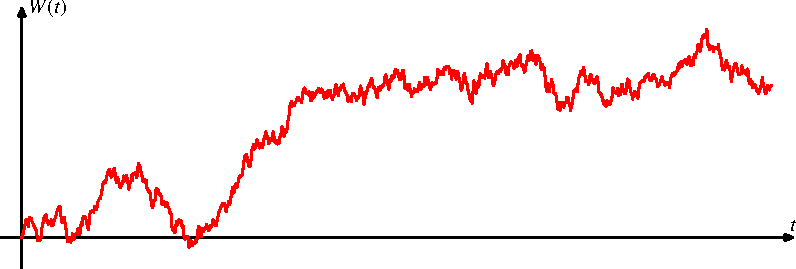
\includegraphics{chapters/images/stochastisch-1.pdf}
\caption{Wiener-Prozess $W(t)$ in Abh"angigkeit von der Zeit
\label{stochastisch:wiener}}
\end{figure}

\subsection{Konstruktion des Wiener-Prozesses}
Wir m"ussen eine Konstruktion angeben, mit der wir zu einem gegebenen
Interval $[0,T]$ eine Funktion $W(t)$ konstruieren k"onnen, die
die Eigenschaften des Wiener-Prozesses erf"ullt.

Zun"achst verlangen die Eigenschaften~1 und 2 des Wiener-Prozesses,
dass $X(T)$ eine normalverteilte Zufallsvariable ist mit Erwartungswert
$X(0)=0$ und Varianz $T$.
Da $X(t)$ ausserdem stetig sein soll, verwenden wir als erste Iteration
die lineare Funktion:
\[
W_1(t) = X(T)\frac{t}{T}
\]
Die Eigenschaft~3 verlangt, dass auch $X(T/2)$ normalverteilt ist mit
Erwartungswert $0$ und Varianz $T/2$.
Dies kann dadurch erreicht werden, dass wir $W_1$ durch einen 
Polygonzug $W_2$ ersetzen, der bei $t=T/2$ einen zus"atzlichen
Eckpunkt besitzt.
Wir bezeichnen den Unterschied zwischen $W_2$ und $W_1$ an der
Stelle $t=T/2$ mit
\[
Y=W_2(T/2)-W_1(T/2)=W_2(T/2) - W_1(T)/2.
\]
$Y$ muss so gew"ahlt werden, dass $W_2(T/2)$ eine normalverteilte
Zufallsvariable mit Erwartungswert $0$ und Varianz $T/2$ wird,
somit ist $Y$ auch normalverteilt.
Der Erwartungswert von $Y$ ist
\begin{align*}
E(Y)&=E(W_2(T/2) - W_1(T)/2)=E(W_2(T/2))-E(W_1(T))/2=0,
\end{align*}
es ist also nur noch die Varianz $\sigma^2_Y$ w"ahlbar.
Sie muss so gew"ahlt werden, dass $W_2(T/2)$ Varianz $T/2$
bekommt:
\begin{align*}
\operatorname{var}\biggl(W_2\biggl(\frac{T}2\biggr))\biggr))
&=
\operatorname{var}\biggl(W_1\biggl(\frac{T}2\biggr) + Y\biggr)
=
\frac{\operatorname{var}(W_1)}4 + \operatorname{var}Y
=
\frac{T}4 +\sigma_Y^2
\end{align*}
Es folgt $\sigma_Y^2=\frac{T}4$.

Wir m"ussen kontrollieren, ob die Inkremente unabh"angig sind.
Dazu berechnen wir der Erwartungswert des Produktes der
beiden Inkremente
\begin{align*}
W_2(T)-W_2\biggl(\frac{T}2\biggr)
&=
W_1(T)-\biggl(\frac{W_1(T)}2 + Y\biggr)
=
Y-\frac{W_1(T)}2
\\
W_2\biggl(\frac{T}2\biggr)-W_2(0)
&=
Y+
\frac{W_1(T)}2
\\
\biggl(W_2(T)-W_2\biggl(\frac{T}2\biggr)\biggr)
\biggl(W_2\biggl(\frac{T}2\biggr)-W_2(0)\biggr)
&=
\biggl(Y-\frac{W_1(T)}2\biggr)\biggl(Y+\frac{W_1(T)}2\biggr)
=
Y^2-\frac{W_1(T)^2}4
\\
E\biggl(
\biggl(W_2(T)-W_2\biggl(\frac{T}2\biggr)\biggr)
\biggl(W_2\biggl(\frac{T}2\biggr)-W_2(0)\biggr)
\biggr)
&=
E(Y^2)-E\biggl(\frac{W_1(T)^2}4\biggr)
=
\sigma_Y^2 - \frac14\operatorname{var}(W_1(T))
=
0
\end{align*}
Somit sind die Inkremente unabh"angig.

\begin{figure}
\centering
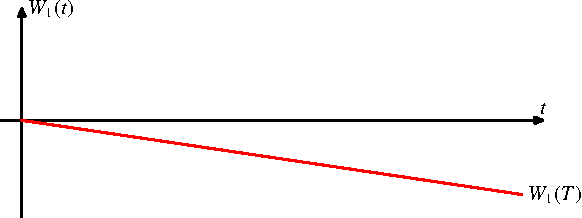
\includegraphics{chapters/images/stochastisch-3.pdf}\\
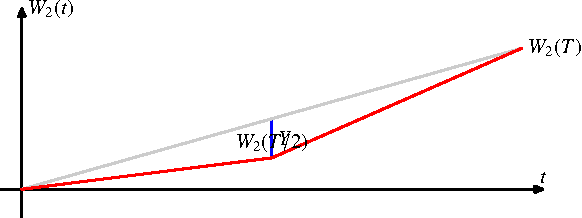
\includegraphics{chapters/images/stochastisch-4.pdf}\\
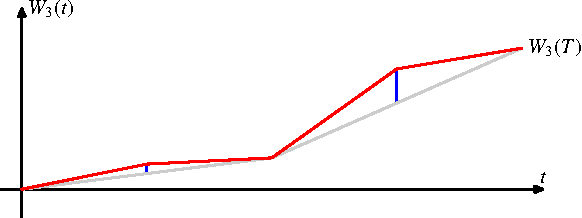
\includegraphics{chapters/images/stochastisch-5.pdf}\\
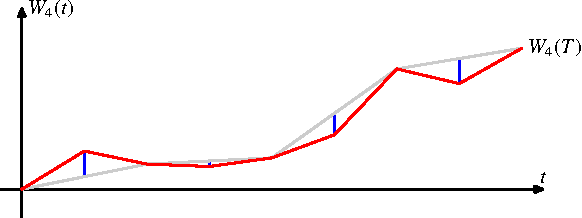
\includegraphics{chapters/images/stochastisch-6.pdf}\\
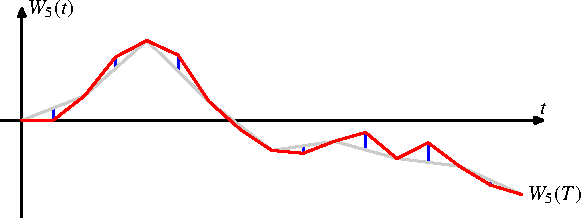
\includegraphics{chapters/images/stochastisch-7.pdf}
\caption{Schrittweise Konstruktion des Wiener-Prozesses als Grenzewert
der Folge $W_n(t)$, $n=1,\dots,5$
\label{stochastisch:folge1}}
\end{figure}
\begin{figure}
\centering
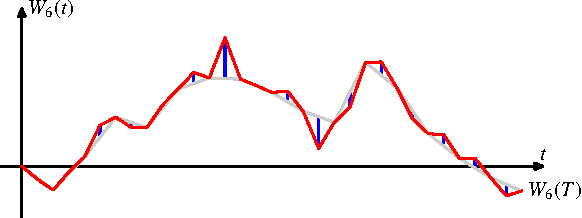
\includegraphics{chapters/images/stochastisch-8.pdf}\\
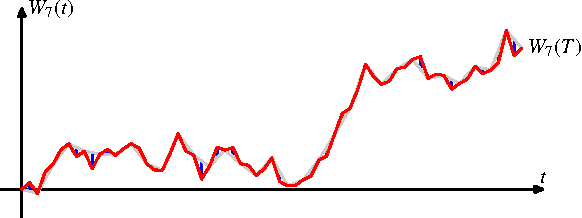
\includegraphics{chapters/images/stochastisch-9.pdf}\\
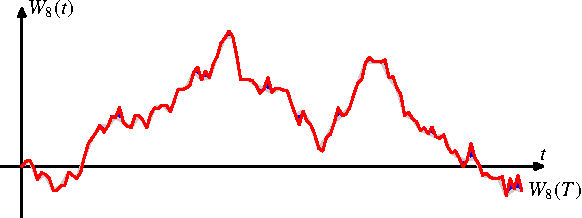
\includegraphics{chapters/images/stochastisch-10.pdf}\\
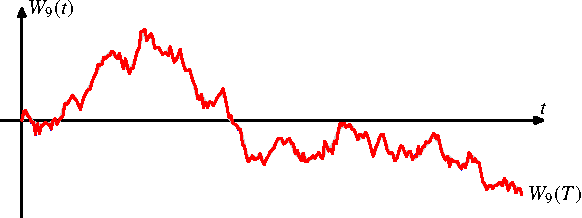
\includegraphics{chapters/images/stochastisch-11.pdf}\\
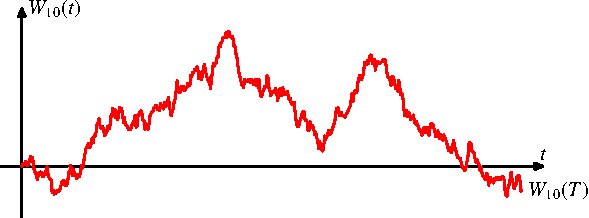
\includegraphics{chapters/images/stochastisch-12.pdf}
\caption{Schrittweise Konstruktion des Wiener-Prozesses als Grenzewert
der Folge $W_n(t)$, $n=6,\dots,10$
\label{stochastisch:folge2}}
\end{figure}

Diesen Prozess k"onnen wir fortsetzen: f"ur $W_3$ nehmen wir einen
Polygonzug mit zus"atzlichen Eckpunkten an den Stellen $T/4$ und $3T/4$.
Die Differenz zwischen $W_3$ und $W_2$ an diesen Stellen m"ussen
normalverteilt sein mit Erwartungswert $0$ und Varianz $T/8$.
Auf diese Weise k"onnen wir eine Folge $W_n$ von Prozessen konstruieren,
wie in den Abbildungen~\ref{stochastisch:folge1} und \ref{stochastisch:folge2}
dargestellt.

Dies reicht aber nicht.
F"ur eine vollst"andige Konstruktion muss man noch die folgenden zwei
Dinge zeigen.
\begin{compactenum}
\item
Der Grenzwert existiert tats"achlich.
Weil die einzelnen Zufallsvariablen $Y$ normalverteilt sind, k"onnen
sie beliebig grosse Werte annehmen.
Dies bedeutet auch, dass wir im Allgemeinen nicht davon ausgehen 
k"onnen, dass die Folge $W_n(t)$ konvergiert.
Zwar sind die Werte von $W_m$ an den Stellen $t_{k,n}=kT/2^{n-1}$ f"ur
$k=0,\dots,2^{n-1}$ fest, sobald $m\ge n$.
Zwischen diesen Werten k"onnen aber immer wieder grosse Werte auftreten,
so dass die Folge $W_n$ weder gleichm"assig noch punktweise konvergieren
kann.
Die Frage der Konvergenz muss daher als Konvergenz in einer Art Mittel 
angegangen werden.
\item
Die Forderung, dass die Inkremente $W(t)-W(s)$ und $W(s)-W(r)$ f"ur jedes 
Tripel $t \ge s\ge r$ unabh"angig sein m"ussen.
Die Konstruktion stellt nur sicher, dass dies gilt, wenn die Zeitpunkte
des Tripels Eckpunkte der Polygonkonstruktion sind.
\end{compactenum}

%
%
%
\section{Stochastische Differentialgleichungen\label{section:stochdgl}}
\rhead{Differentialgleichungen}
Wir m"ochten gerne eine Differentialgleichung f"ur den Zustand
$X(t)$ eines Systems l"osen, welches von Rauschen mit beeinfluss wird.
Eine solche Differentialgleichung k"onnten wir schreiben als
\[
\frac{dX(t)}{dt}
=
b(X(t)) + B(X(t))\frac{dW(t)}{dt}
\]
wobei $b$ die Rolle der Funktion $f$ aus
Abschnitt~\ref{section:anfangswertprobleme} spielt.
Die Ableitung von $W$ spielt die Rolle des Rauschens, wir wissen aber
bereits, dass $W$ nicht differenzierbar sein kann, die Gleichung
in dieser Form kann daher gar nicht sinnvoll sein.

Formal kann man die Gleichung mit $dt$ multiplizieren, so dass man
das formale Gleichungssystem
\begin{align*}
dX(t)
&=
b(X(t)) + B(X(t),t)\,dW(t)
\\
X(0)
&=
x_0
\end{align*}
erh"alt, aber auch in diesr Form sind die Ausdr"ucke $dX$ und $dW$ nicht
ohne zus"atzliche Definition sinnvoll.
Am ehesten hat man eine Chance, dieser Gleichung einen Sinn zu geben,
wenn man integriert:
\begin{align*}
X(t)=x_0+\int_0^t b(X(s))\,ds + \int_0^t B(X(s), s)\, dW,\qquad t>0.
\end{align*}
Das erste Integral ist ein gew"ohnliches Integral, denn wir
gehen davon aus, dass die Funktion $X(t)$ stetig ist.
Wenn $B=0$ ist, dann liefert diese Formel genau L"osungen der
urspr"unglichen Differentialgleichung.
Wir brauchen aber immer noch eine Interpretation des zweiten Integrals,
diese werden wir in Abschnitt~\ref{subsection:stochint} geben.

Nehmen wir f"ur den Moment an, dass die L"osung $X(t)$ gefunden werden
kann, und sei $u$ eine beliebig oft differenzierbare Funktion.
Wir erwarten, dass die Ableitung von $Y(t)=u(X(t))$ nach der
Kettenregel
\[
dY = u'\,dX = u'b\,dt + u'\,dW
\]
sein sollte.
Tats"achlich ist das Rauschen so stark, dass die Kr"ummung der Funktion
$u$ bereits eine Rolle spielt.
Bei einer gew"ohnlichen Differentialgleichung sind auf kleine Entfernungen
die zweiten Ableitungen von $u$ vernachl"assigbar.
Die schnellen, vom Rauschen verursachten Abweichungen f"uhren sind aber nicht
klein, so dass die korrekte Kettenregel bei Anwesenheit von Rauschen die
It\^o-sche Kettenregel wird, die stattdessen den Ausdruck
\[
dY =  \biggl(u'b + \frac12u''\biggr)\,dt + u'\,dW
\]
liefert.
Der Term $\frac12u''$ ist in der klassischen Analysis nicht vorhanden.
Wir m"ussen daher auch alle gewohnten Rechenregeln der Analysis "uberpr"ufen.

\subsection{Stochastische Integrale\label{subsection:stochint}}
\index{stochastisches Integral}
Wir m"ochten eine Definition f"ur ein Integral der Form
\[
\int_0^T G\,dW
\]
f"ur zwei stochastische Prozesse $G(t)$ und $W(t)$.

\subsubsection{Das Paley-Wiener-Zygmund Integral}
\index{Paley-Wiener-Zygmund Integral}
F"ur differenzierbare Funktionen $g(t)$ und $w(t)$ ist klar, was 
mit dem Integral gemeint ist:
\[
\int_0^T g(t)\,dw = \int_0^T g(t) w'(t)\,dt.
\]
Wenn $g(0)=g(T)=0$ ist, dann kann man dies mit Hilfe partieller Integration
vereinfachen:
\[
\int_0^T g(t)\,dw
=
\int_0^T g(t) w'(t)\,dt
=
[g(t)w(t)]_0^T
-
\int_0^T g'(t) w(t)\,dt
=
-\int_0^T g'(t) w(t)\,dt
\]
Diese letzte Formel ist aber auch geeignet als Definition des Integrals
f"ur eine brownsche Bewegung $W(t)$ an Stelle von $w(t)$.

\begin{definition}
F"ur eine stetig differenzierbare Funktion $g\colon[0,T]\to \mathbb R$ 
mit $g(0)=g(T)=0$, setze
\[
\int_0^T g\,dW = -\int_0^T g'(t) W(t)\,dt.
\]
\end{definition}

\begin{hilfssatz}
Erwartungswert und Varianz der Zufallsvariablen
\[
Z=\int_0^T g\,dW
\]
ist
\begin{compactenum}
\item $E(Z)=0$
\item $\operatorname{var}(Z)=\int_0^Tg(t)^2\,dt$
\end{compactenum}
\end{hilfssatz}

\begin{proof}[Beweis]
F"ur den Erwartungswert finden wir mit Hilfe der Rechenregeln f"ur den
Erwartungswert
\begin{align*}
E(Z)
&=
E\biggl(\int_0^T g\,dW\biggr)
=
E\biggl(
\int_0^T g'(t) W(t)\,dt
\biggr)
=
\int_0^T g'(t) \underbrace{E(W(t))}_{\textstyle =0}\,dt=0
\end{align*}
Die Varianz ist daher der Erwartungswert $E(Z^2)$, die wir ebenfalls unter
Verwendung der Rechenregeln berechnen k"onnen
\begin{align*}
E(Z^2)
&=
E\biggl(\biggl(\int_0^T g\,dW\biggr)^2\biggr)
=
E\biggl(
\biggl(
\int_0^T g'(t)W(t)\,dt
\biggr)^2
\biggr)
\\
&=
E\biggl(
\int_0^T g'(t)W(t)\,dt
\int_0^T g'(s)W(s)\,ds
\biggr)
=
E\biggl(
\int_0^T \int_0^T g'(t)W(t) g'(s)W(s) \,ds \,dt
\biggr)
\\
&=
\int_0^T\int_0^Tg'(t)g'(s) \underbrace{E(W(t)W(s))}_{\textstyle =t\wedge s}\,ds\,dt
\\
&=
\int_0^Tg'(t) \biggl(\int_0^t g'(s) s\,ds + \int_t^T g'(s)t\,ds\biggr)
\,dt
\\
&=
\int_0^T g'(t)\biggl(
\underbrace{[g(s)s]_0^t}_{\textstyle =tg(t)}-\int_0^t g(s)\,ds+t(\underbrace{g(T)}_{\textstyle =0}-g(t))
\biggr)\,dt
\\
&=
\int_0^T g'(t)\biggl(-\int_0^t g(s)\,ds\biggr)\,dt
\\
&=
\biggl[
g(t)\biggl(-\int_0^t\int_0^tg(s)\,ds\biggr)
\biggr]_0^T
+
\int_0^Tg(t)^2\,dt
\end{align*}
Damit ist die Behauptung bewiesen.
\end{proof}
Der Hilfssatz kann dazu verwendet werden, die Definition des Integrals auf
weitere Funktionen auszudehnen.
Eine Folge von Funktionen $g_n$ f"uhrt auf eine Folge von Werten des
Integrals. 
Um daraus eine Erweiterung des Integrals zu konstruieren, m"ussen wir 
definieren, was es heissen soll, dass die Folge $g_n$ konvergiert.
Wir verwenden die Norm
\[
\|f\|_2^2=\int_0^T f(t)^2 \,dt,
\]
um den Abstand zwischen Funktionen zu messen.
Eine Cauchy-Folge von Funktionen in dieser Norm ist dann eine Folge so,
dass f"ur jedes $\varepsilon>0$ ein $N>0$ existiert, so dass aus
$n,m>N$ folgt
\[
\|g_n-g_m\|_2^2=\int_0^T (g_n(t)-g_m(t))^2\,dt<\varepsilon.
\]
In diesem Fall gilt, dass
\[
E\biggl(
\biggl(
\int_0^T g_n\,dW
-
\int_0^T g_m\,dW
\biggr)^2
\biggr)
=
\int_0^T(g_m(t)-g_n(t))^2\,dt<\varepsilon
\]
Die Zufallsvariablen
\[
Z_n = \int_0^T g_n\,dW
\]
bildet daher eine Cauchy-Folge von quadratintegrierbaren Funktionen
in $L^2(\Omega)$, und wir k"onnen deren Grenzwert
\[
\int_0^T g\,dW
=
\lim_{n\to\infty}\int_0^T g_n\,dW
\]
als den verallgemeinerten Wert f"ur das Integral einer beliebigen Funktion
$g\in L^2([0,T])$ definieren.

\subsubsection{Riemann-Summen}
Die Verallgemeinerung des Paley-Wiener-Zygmund-Integral auf
quadratintegrierbare Funktionen ist allerdings nicht ausreichend, um
\[
\int_0^T W\,dW
\]
zu definieren.
Wir k"onnen aber noch weiter zur"uck gehen zur Definition des
Riemann-Integrals, und sie verallgemeinern auf einen stochastischen
Prozess.

\begin{definition}
Eine {\em Unterteilung} $P$ des Intevals $[0,T]$ ist eine endliche Menge
von Teilpunkten
\[
P=\{ 0=t_0<t_1<t_2<\dots<t_m=T\}.
\]
Die {\em Maschenweite} $|P|$ der Unterteilung $P$ ist
\[
|P|=\max_{0\le k\le m-1}|t_{k+1\mathstrut}-t_{k\mathstrut}|.
\]
F"ur ein festes $0\le \lambda\le 1$ setzen wir
\[
\tau_k = (1-\lambda)t_{k\mathstrut}+\lambda t_{k+1\mathstrut}.
\]
\end{definition}
F"ur $\lambda=0$ ist $\tau_k=t_k$, f"ur $\lambda=1$ gilt $\tau_k=t_{k+1}$.
F"ur andere Werte von $\lambda$ ist $\tau_k$ ein Punkt im Inneren des
Intervals $[t_k,t_{k+1}]$.
Wie "ublich kann eine solche Unterteilung dazu verwendet werden, die 
Riemann-Summe als Approximation des Integrals zu definieren:

\begin{definition}
Die Riemann-Summe von f"ur $\int W\,dW$ und die Unterteilung $P$ ist
\[
R=R(P,\lambda) = \sum_{k=0}^{m-1} W(\tau_k)(W(t_{k+1})-W(t_k)).
\]
\index{Riemann-Summe}
\end{definition}

\begin{hilfssatz}
\label{stochastisch:quadrvariation}
Sei
\[
P^{(n)}
=
\{0=t_0^{(n)}<t_1^{(n)}<\dots < t_{m_n}^{(n)}=T\}
\]
eine Folge von Unterteilungen des Intervals $[0,T]$ derart,
dass die Maschenweite gegen $0$ strebt, dann gilt
\[
\lim_{n\to\infty}
\sum_{k=0}^{m_n-1} \bigl(W(t_{k+1}^{(n)})-W(t_{k}^{(n)})\bigr)^2
=T
\]
in $L^2(\Omega)$.
\end{hilfssatz}

\begin{proof}[Beweis]
Konvergenz in $L^2(\Omega)$ bedeutet, dass der Erwartungswert der
quadratische Abweichung gegen $0$ streibt.
Setzen wir
\[
Q_n
= 
\sum_{k=0}^{m_n-1} \left(W(t_{k+1}^{(n)})-W(t_{k}^{(n)})\right)^2,
\]
und m"ussen untersuchen, ob $E((Q_n - T)^2)$ gegen $0$ strebt.
Wir beginnen mit der Bemerkung, dass
\begin{align*}
Q_n-T
&=
\sum_{k=0}^{m_n-1}
\left((W(t_{k+1}^{(n)})-W(t_{k}^{(n)}))^2 - (t_{k+1}^{(n)}-t_k^{(n)})\right).
\end{align*}
Die einzelnen Differenzen k"urzen wir ab als
\begin{align*}
Y_k
&=
\frac{W(t_{k+1}^{(n)})-W(t_k^{(n)})}{\sqrt{t_{k+1}^{(n)}-t_{k}^{(n)}}},
\\
\Delta_k
&=
t_{k+1}^{(n)}-t_k^{(n)}.
\end{align*}
F"ur $j\ne k$ sind $Y_j^{(n)}$ und $Y_{k}^{(n)}$ unabh"angig.
Ausserdem ist $Y_k$ standardnormalverteilt, also $E(Y_k)=0$
und $E(Y_k^2)=1$.
Die Summanden in der Summe lassen sich damit kompakter ausdr"ucken:
\begin{align*}
Q_n-T
&=
\sum_{k=0}^{m_n-1} (Y_k^2-1) \Delta_k
\end{align*}
Dies k"onnen wir in $E((Q_n-T)^2)$ einsetzen:
\begin{align*}
E((Q_n-T)^2)
&=
\sum_{k=0}^{m_n-1}
\sum_{j=0}^{m_n-1}
E\biggl(
(Y_k^2-1)\Delta_k
(Y_j^2-1)\Delta_j
\biggr)
\end{align*}
Die Doppelsumme kann zerlegt werden in Terme mit $j=k$ und $j\ne k$.

In den Terme mit $j\ne k$ sind die $Y_k$ und $Y_j$ voneinander unabh"angig,
der Erwartungswert des Produktes kann daher in das Produkt der Erwartungswerte
zerlegt werden:
\begin{align*}
E\left(
(Y_k^2-1)\Delta_k
(Y_j^2-1)\Delta_j
\right)
&=
E(Y_k^2-1)
E(Y_j^2-1)
\Delta_k
\Delta_j
\\
&=
\bigl(E(Y_k^2) -1\bigr)
\bigl(E(Y_j^2) -1\bigr)
\Delta_k
\Delta_j
=0
\end{align*}
Im letzten Schritt haben wir verwendet, dass $E(Y_k^2)=\operatorname{var}Y_k=1$
ist.

Die Terme mit $j=k$ sind 
\begin{align*}
E((Q_n-T)^2)
&=
\sum_{k=0}^{m_n-1} E\biggl((Y_k^2-1)^2\Delta_k^2\biggr)
\\
&=
\sum_{k=0}^{m_n-1} E\bigl((Y_k^2-1)^2\bigr)\Delta_k^2
\le 
\biggl(\sum_{k=0}^{m_n-1} E\bigl((Y_k^2-1)^2\bigr)\Delta_k\biggr)\, |P^{(n)}|
\end{align*}
Im letzten Schritt haben wir einen Faktor $\Delta_k$ aus der Summe
herausgenommen und durch die Maschenweite $|P^{(n)}|$ abgesch"atzt.

Da $Y_k$ standardnormalverteilt ist, ist der Erwartungswert $E((Y_k^2-1)^2)$
unabh"angig von $k$, wir nennen diesen Wert $C$, der genaue Wert ist
nicht wichtig\footnote{Man kann den Wert nat"urlich wie folgt berechnen:
\begin{align*}
E((Y_k^2-1)^2)
&=
E(Y_k^4-2Y_k^2+1)
=
E(Y_k^4)-2E(Y_k^2)+E(1)
=
6-2+1=5.
\end{align*}}.
Damit l"asst sich die Differenz jetzt unabh"angig von $k$ absch"atzen
\begin{align*}
E((Q_n-T)^2)
&
\le
C\biggl(\sum_{k=1}^{m_n}\Delta_k\biggr)\, |P^{(n)}|
=CT|P^{(n)}|.
\end{align*}
Da die Maschenweite $|P^{(n)}|\to 0$ f"ur $n\to\infty$ folgt, dass
$Q_n\to T$ in $L^2(\Omega)$.
\end{proof}

\begin{hilfssatz}
\label{stochastisch:intwdw}
Sei $P^{(n)}$ eine Folge von Unterteilungen des
Intervals $[0,T]$ derart, dass die Maschenweite gegen $0$ strebt und
sei $R_n=R(P^{(n)},\lambda)$ die zugeh"orige Riemann-Summe.
Dann gilt
\[
\lim_{n\to\infty} R_n = \frac{W(T)^2}2 + \biggl(\lambda-\frac12\biggr)T
\]
als Funktion in $L^2(\Omega)$.
\end{hilfssatz}

\begin{proof}[Beweis]
Wir m"ussen die Riemann-Summe
\begin{align*}
R_n
&=
\sum_{k=0}^{m_n-1}
W(\tau_k) (W(t_{k+1}^{(n)})-W(t_k^{(n)}))
\end{align*}
durch Inkremente von Werten von $W(t)$ ausdr"ucken, konkret durch
\[
W(t_{k+1}^{(n)})-W(t_k^{(n)}),\quad
W(t_{k+1}^{(n)})-W(\tau_k^{(n)})
\quad \text{und} \quad
W(\tau_k^{(n)})-W(t_k^{(n)}).
\]
Um herauszufinden, wie dies m"oglich sein k"onnte, k"urzen wir die Werte
von $W$ ab durch
\[
a_k=W(t_k^{(n)}),\quad
b_k=W(\tau_k^{(n)})\quad\text{und}\quad
c_k=W(t_{k+1}^{(n)}),
\]
wobei wir im folgenden zur Vereinfachung der Rechnung die Indizes auch
weglassen.
Jetzt versuchen wir $b(c-a)$ durch andere Differenzen auszudr"ucken.
\begin{align*}
(b-a)^2
&=
b^2-2ab + a^2
\\
(c-a)^2
&=
c^2-2ac+a^2
\\
(c-b)(b-a)
&=
cb-b^2-ac+ab
\end{align*}
Um den Ausdruck $b(c-a)$ zu produzieren, muss der letzte Term verwendet
werden, denn er ist der einzige, der $bc$ enth"alt.
Dann muss aber auch der erste Term verwendet werden, um den Term $b^2$ zum
Verschwinden  zu bringen.
Ebenso muss der zweite Term $\frac12$-mal subtrahiert werden, damit der
Ausdruck $ac$ wegf"allt:
\begin{align*}
(b-a)^2-\frac12(c-a)^2+(c-b)(b-a)
&=
(b^2-2ab + a^2)
-\frac12(c^2-2ac+a^2)
+(cb-b^2-ac+ab)
\\
&=
cb-ab + \frac12a^2
-\frac12c^2
\end{align*}
Die quadratischen Terme sind $\frac12c_k^2=\frac12W(t_{k+1}^{(n)})^2$ und
$\frac12a_k^2=\frac12W(t_{k}^{(n)})^2$, die sich in aufeinanderfolgenden Termen
jeweils wegheben.
Nur der erste und letzte Term bleibt in der Summe bestehen, was wir
aber leicht korrigieren k"onnen.
So finden wir daher:
\begin{align*}
R_n
&=
\underbrace{
\sum_{k=0}^{m_n-1} (b_k-a_k)^2
}_{\textstyle\to\lambda T}
-
\underbrace{
\frac12\sum_{k=0}^{m_n-1} (c_k-a_k)^2
}_{\textstyle\to T}
+\sum_{k=0}^{m_n-1} (c_k-b_k)(b_k-a_k)
- \frac12a_0^2
+ \frac12c_{m_n-1}^2
\end{align*}
Die zweite Summe wurde im Hilfssatz~\ref{stochastisch:quadrvariation}
berechnet, dort wurde gefunden, dass die Summe f"ur $n\to\infty$ gegen $T$
konvergiert.
Mit der gleichen Rechnung wie in \ref{stochastisch:quadrvariation}
kann man finden, dass die erste Summe gegen $\lambda T$ strebt.

Die Inkremente in der dritten Summe sind unabh"angig voneinander, daher
verschwinden die Erwartunsgewerte gemischter Produkte, es bleiben nur
die Terme
\begin{align*}
E\biggl(\biggl(\sum_{k=0}^{m_n-1}(c_k-b_k)(b_k-a_k)\biggr)^2\biggr)
&=
\sum_{k=0}^{m_n-1}
E\bigl((c_k-b_k)^2\bigr)E\bigl((b_k-a_k)^2\bigr)
\\
&=
\sum_{k=0}^{m_n-1}
E\bigl((W(t_{k+1}^{(n)})-W(\tau_k^{(n)}))^2\bigr)E\bigl((W(\tau_k^{(n)})-W(t_k^{(n)})^2\bigr)
\\
&=
\sum_{k=0}^{m_n-1}
(t_{k+1}^{(n)}-\tau_k^{(n)}) (\tau_k^{(n)}-t_k^{(n)})
\\
&=
\sum_{k=0}^{m_n-1}
(1-\lambda)(t_{k+1}^{(n)}-t_k^{(n)}) \lambda(t_{k+1}^{(n)}-t_k^{(n)})
\\
&\le 
(1-\lambda)\lambda
|P^{(n)}|
\sum_{k=0}^{m_n-1}
(t_{k+1}^{(n)}-t_k^{(n)})
\le (1-\lambda)\lambda T|P^{(n})|\to 0
\end{align*}
f"ur $n\to\infty$.
Damit ist gezeigt, dass die Riemann-Summe in $L^2(\Omega)$ gegen
\[
R_n\to
\frac{W(T)^2}2+\biggl(\lambda-\frac12\biggr)T
\]
konvergiert.
\end{proof}

\subsubsection{Das It\^o-Integral}
Ausgehend von der Riemann-Summe und den f"ur sie hergeleiteten Eigenschaften
wollen wir jetzt ein Integral
\[
\int_0^T G\,dW
\]
f"ur eine breitere Klasse von stochastischen Prozessen $G$ definieren.
Der erste Schritt dazu, ist das Integral f"ur Stufenprozesse zu definieren.

\begin{definition}
\index{Stufenprozess}
Ein stochastischer Prozess $G(t)$ ist eine {\em Stufenprozess}, wenn es eine
Unterteilung $P=\{0=t_0<t_1<\dots<t_m=T\}$ gibt derart, dass
$G(t)=G(t_k)$ f"ur $t_k\le t<t_{k+1}$.
\end{definition}

\begin{definition}
Ist $G$ ein Stufenprozess, dann ist das {\em It\^o-Integral} von $G$ definiert
als
\[
\int_0^TG\,dW = \sum_{k=0}^{m-1}G(t_k)(W(t_{k+1})-W(t_k)).
\]
Das It\^o-Integral ist eine Zufallsvariable.
\end{definition}

Das It\^o-Integral hat die folgenden Eigenschaften
\begin{hilfssatz}
Wenn $G$ und $H$ Stufenprozesse sind und $a,b\in\mathbb R$, dann gilt
\begin{compactenum}
\item Das It\^o-Integral ist linear:
\[
\int_0^T aG+bH\,dW
=
a\int_0^T G\,dW + b \int_0^TH\,dW
\]
\item Der Erwartungswert des It\^o-Integrals ist $0$:
\[
E\biggl(\int_0^T G\,dW\biggr)=0.
\]
\item Die Varianz des It\^o-Integrals ist
\[
E\biggl(\biggl(\int_0^T G\,dW\biggr)^2\biggr)
=
E\biggl(\int_0^T G^2\,dt\biggr)
\]
\end{compactenum}
\end{hilfssatz}

\begin{proof}[Beweis]
F"ur die Linearit"at verwenden wir eine Unterteilung $P$, f"ur die sowohl
$G$ also auch $H$ ein ein Stufenprozess ist.
Dann gilt
\begin{align*}
\int_0^T aG+bH\,dW
&=
\sum_{k=0}^{m-1} (aG(t_k)+bH(t_k))(W(t_{k+1})-W(t_k))
\\
&=
a\sum_{k=0}^{m-1} G(t_k)(W(t_{k+1})-W(t_k))
+
b\sum_{k=0}^{m-1} H(t_k)(W(t_{k+1})-W(t_k))
\\
&=a\int_0^TG\,dW+b\int_0^TH\,dW
\end{align*}
womit die Linearit"at bewiesen ist.

F"ur den Erwartungswert berechnen wir mit Hilfe einer passenden Unterteilung
\begin{align*}
E\biggl(\int_0^T G\,dW\biggr)
&=
E\biggl(\sum_{k=0}^{m-1} G(t_k) (W(t_{k+1}) - W(t_k))\biggr)
\\
&=
\sum_{k=0}^{m-1} E(G(t_k)) \underbrace{E(W(t_{k+1}) - W(t_k))}_{\textstyle =0}=0.
\end{align*}
Damit ist 2.~beweisen.

F"ur die Berechnung der Varianz verwendet wieder die Unabh"angigkeit der
Inkremente:
\begin{align*}
E\biggl(\biggl(\int_0^T G\,dW\biggr)^2\biggr)
&=
E\biggl(\biggl(\sum_{k=0}^{m-1}G(t_k)(W(t_{k+1})-W(t_k))\biggr)^2\biggr)
\\
&=
E\biggl(
\sum_{k=0}^{m-1}G(t_k)(W(t_{k+1})-W(t_k))
\sum_{j=0}^{m-1}G(t_j)(W(t_{j+1})-W(t_j))
\biggr)
\\
&=
\sum_{k=0}^{m-1}
\sum_{j=0}^{m-1}
E(G(t_k) G(t_j)
(W(t_{k+1})-W(t_k))
(W(t_{j+1})-W(t_j))
)
\\
&=
\sum_{k=0}^{m-1}
E(G(t_k)^2) E(W(t_{k+1})-W(t_k))^2)
\\
&=
\sum_{k=0}^{m-1}
E(G(t_k)^2) (t_{k+1}-t_k)
=
E\biggl(
\sum_{k=0}^{m-1}
G(t_k)^2 (t_{k+1}-t_k)
\biggr)
=E\biggl(\int_0^T G(t)^2\,dt\biggr).
\end{align*}
Somit ist auch 3.~bewiesen.
\end{proof}

Die Bedeutung der dritten Eigenschaft besteht darin, dass eine
Folge von Stufen-Prozessen, die $L^2(0,T)$ konvergiert, zu einer
konvergenten Folge von It\^o-Integralen f"uhrt.

\begin{definition}
\index{It\^o-Integral}
Ist $G$ ein beliebiger auf $[0,T]$ quadratintegrierbarer Prozess,
und $G_n$ eine Folge von stochastischen Prozessen, die in $L^2([0,T])$
gegen $G$ konvergiert.
Dann ist des It\^o-Integral von $G$
\[
\int_0^T G\,dW
=
\
\lim_{n\to\infty} \int_0^T G_n\,dW
\]
\end{definition}

\begin{beispiel}
Wir haben die Riemann-Summe f"ur $G=W$ bereits in
Hilfssatz~\ref{stochastisch:intwdw} berechnet, daher k"onnen wir jetzt
das It\^o-Integral angeben:
\[
\int_0^t W\,dW
=
\frac12 W(t)^2 -\frac{t}2.
\]
In differentieller Form:
\[
d(W^2)
=
2W\,dW + t.
\]
Dies ist ein Spezialfall der sp"ater zu untersuchenden It\^o-Produktregel.
\end{beispiel}

Das It\^o-Integral hat die folgenden Eigenschaften:

\begin{satz}
\label{satz:ito-integral}
Seien $G$ und $H$ auf $[0,T]$ quadratintegrierbare stochastische Prozesse
und $a,b\in\mathbb R$. Dann gilt
\begin{compactenum}
\item Das It\^o-Integral ist linear:
\[
\int_0^T aG+bH\,dW
=
a\int_0^TG\,dW
+
b\int_0^TH\,dW
\]
\item Der Erwartungswert des It\^o-Integrals ist
\[
E\biggl(\int_0^T G\,dW\biggr)=0
\]
\item Die Varianz des It\^o-Integrals ist
\[
E\biggl(\biggl(\int_0^TG\,dW\biggr)^2\biggr)
=
E\biggl(\int_0^T G^2\,dt\biggr).
\]
\end{compactenum}
\end{satz}

Mit dem It\^o-Integral k"onnen wir jetzt alle Komponenten einer
stochastischen Differentialgleichung definieren.
Zun"achst k"onnen wir f"ur jeden auf $[0,T]$ quadratintegrierbaren Prozess $G$ 
und f"ur jede integrierbare Funktion $F\in L^1([0,T])$ die Gr"ossen
\begin{align*}
\int_s^r F(t)\,dt&=\int_0^r F(t)\,dt - \int_0^s F(t)\,dt
\\
\int_s^r G\,dW&=\int_0^r G\,dW - \int_0^s G\,dW
\end{align*}
definieren.
\begin{definition}
Wenn $X$ ein stochastischer Prozess ist, der
\[
X(r)=X(s)+\int_s^rF(t)\,dt + \int_s^tG\,dW
\]
erf"ullt, dann sagt man $X$ habe das {\em stochastische Differential}
\[
dX=F\,dt + G\,dW.
\]
\end{definition}

%
%
%
\subsection{Rechenregeln}
Bisher wissen wir nur, dass das It\^o-Integral linear ist, dies reicht
aber nicht f"ur einen Kalk"ul, mit dem wir hoffen k"onnen,
Differentialgleichungen zu l"osen.u
Dazu brauchen wir mindestens noch eine Kettenregel und eine
Produktregel.

\begin{satz}[It\^o's Kettenregel]
\index{It\^o-Kettenregel}
Falls $X$ das stochastische Differential
\[
dX=F\,dt + G\,dW
\]
hat, und falls $u\colon \mathbb R\times [0,T]\to\mathbb R$ eine
stetig differenzierbare Funktion.
Dann hat die Funktion $Y(t)=u(X(t), t)$ das stochastische Differential
\begin{align*}
du(X,t)
&=\frac{\partial u}{\partial t}\,dt + \frac{\partial u}{\partial x}\,dX 
+\frac12\frac{\partial u^2}{\partial x^2}G^2\,dt
\\
&=
\biggl(
\frac{\partial u}{\partial t}+\frac{\partial u}{\partial x}F
+\frac12\frac{\partial^2u}{\partial x^2}G^2
\biggr)\,dt
+
\frac{\partial u}{\partial x}G\,dW.
\end{align*}
\end{satz}
Bis auf den Term in den zweiten Ableitungen sind die Terme genau
diejenigen, die man von der klassischen Kettenregel her erwarten
k"onnte.

\begin{beispiel}
Potenzen eines Wiener-Prozesses.
Sei $u(x)=x^m$ und $X=W$, $F=0$ und $G=1$.
Also ist $Y=W^m$.
Dann hat nach der It\^o-schen Kettenregel das stochastische Differential
\[
d(W^m)
=
\frac12m(m-1)W^{m-2}\,dt + mW^{m-1}\,dW.
\]
Im Spezialfall $m=2$ folgt
\[
dW^2 = 2W\,dW + dt.
\]
Dies haben wir schon als Resultat von
Hilfssatz~\ref{stochastisch:intwdw} gefunden.
\end{beispiel}

\begin{beispiel} Wir betrachten die Funktion
$u(x,t)=e^{\lambda x-\frac12\lambda^2 t}$, und wie vorhin $X=W$, $F=0$
und $G=1$.
Es folgt
\begin{align*}
d\biggl(
e^{\lambda W(t)-\frac12\lambda^2 t}
\biggr)
&=
\biggl(
-\frac12\lambda^2 e^{\lambda W-\frac12\lambda^2 t}
+
\frac12\lambda^2 e^{\lambda W-\frac12\lambda^2 t}
\biggr)\,dt
+
\lambda e^{\lambda W -\frac12\lambda^2 t}\,dW
\\
dY&=\lambda Y\,dW
\end{align*}
also ist der Prozess $Y$ eine L"osung der stochastischen Differentialgleichung
\begin{align*}
dY&=\lambda Y\,dW
\\
Y(0)&=1.
\end{align*}
Dieses Beispiel zeigt, dass der entwickelte Kalk"ul dazu geeignet sein kann,
stochastische Differentialgleichungen zu l"osen.
\end{beispiel}

\begin{satz}[Produktregel von It\^o]
\index{It\^o-Produktregel}
\index{Produktregel von It\^o}
Falls die Prozesse $X_1$ und $X_2$ die stochastischen Differentiale
\begin{align*}
dX_1
&=
F_1\,dt + G_1\,dW
\\
dX_2
&=
F_2\,dt + G_2\,dW
\end{align*}
haben, dann ist
\begin{equation}
d(X_1X_2)
=
X_2\,dX_1 + X_1\,dX_2 + G_1G_2\,dt,
\label{stochastisch:ito-produkt}
\end{equation}
dies ist die {\em It\^o-sche Produktformel}.
\end{satz}

F"ur den Beweis der Kettenregel brauchen wir die Produktregel, wir geben
daher zuerst einen Beweis f"ur die Produktregel an.

\begin{proof}[Beweis der Produktformel]
Die integrierte Form der Produktregel besagt, dass 
\begin{equation}
X_1(r)X_2(r)-X_1(0)X_2(0)
=
\int_0^r X_2\,dX_1 + \int_0^r X_1\,dX_2 + \int_0^r G_1G_2\,dt
\label{stochastisch:ito-produkt-integriert}
\end{equation}
diese m"ussen wir nachrechnen.
Wir nehmen an der Einfachheit halber an, dass $X_1(0)=X_2(0)=0$ ist.

1.~Wir nehmen zus"atzlich an, dass die Funktion $G_i$ und $F_i$ nicht von
der Zeit abh"angen.
Dies bedeutet, dass sich die stochastische Differentialgleichung
$dX_i=F_i\,dt+G_i\,dW$ integrieren l"asst:
\[
X_i(t) = \int_0^t F_i\,d\tau + G_i\int_0^r dW =  F_it+G_iW(t).
\]
Diese Bedingung werden wir im zweiten Schritt wieder aufheben.
Wir berechnen die rechte Seite der integrierten
Produktregel~(\ref{stochastisch:ito-produkt-integriert}):
\begin{align*}
\int_0^r X_2\,dX_1 + X_1\,dX_2 + G_1G_2\,dt
&=
\int_0^rX_1F_2+X_2F_1\,dt + \int_0^r X_1G_2+X_2G_1\,dW + \int_0^r G_1G_2\,dt
\\
&=
\int_0^r(F_1t+G_1W)F_2+(F_2t+G_2W)F_1\,dt
\\
&\qquad
+ \int_0^r (F_1t+G_1W)G_2+(F_2t+G_2W)G_1\,dW + \int_0^r G_1G_2\,dt
\\
&=F_1F_2r^2+(G_1F_2+G_2F_1)\underbrace{\biggl(\int_0^rW\,dt + \int_0^rt\,dW\biggr)}_{\textstyle = rW(r)}
\\
&\qquad
+G_1G_2\cdot \underbrace{2\int_0^r W\,dW}_{\textstyle W(r)^2-r}
+ G_1G_2\underbrace{\int_0^r\,dt}_{\textstyle =r}
\\
&= 
F_1F_2r^2 + (G_1F_2+G_2F_1)rW(r) + G_1G_2W(r)^2
\\
&= 
F_1r\cdot F_2r + F_2r\cdot G_1W(r)+F_1r\cdot G_2W(r) + G_1W(r)\cdot G_2W(r)
\\
&= 
(F_1r + G_1W(r))\cdot(F_2r +  G_2W(r))
=
X_1(r) \cdot X_2(r).
\end{align*}
Dies ist die linke Seite von (\ref{stochastisch:ito-produkt-integriert}), die
damit f"ur diesen Spezialfall bewiesen ist.

2.~Wir ersetzen jetzt die Konstanten $G_i$ und $F_i$ durch Stufenprozesse.
Es gibt eine Unterteilung des Intervals $[0,T]$ so, dass die Prozesse $G_i$
und $F_i$ in jedem Teilinterval konstant sind.
In jedem solchen Teilinterval gilt daher die Ito-Produktformel, und damit
auch f"ur das ganze Interval.

3.~Im allgemeinen Fall k"onnen wir die Prozesse $G_i$ und $F_i$ mit Hilfe
einer Formel von Stufenprozessen $G_i^n$ und $F_i^n$ approximieren.
Wir k"onnen zus"atzlich fordern, dass
\[
E\biggl(\int_0^T |F_i^n-F_i|\,dt\biggr)\to 0
\qquad\text{und}\qquad
E\biggl(\int_0^T (G_i^n-G_i)^2\,dt\biggr)\to 0,
\]
was wir weiter unten brauchen.
Es gibt nach dem zweiten Schritt eine Folge von Prozessen $X_i^n$ mit
\[
X_i^n(t) = X_i(0) + \int_0^t F_i^n\,d\tau + \int_0^t G_i^n\,dW,
\]
f"ur die jeweils die Produktregel gilt.
\begin{align*}
X_i^n(r)X_i^n(r)-X_i^n(s)X_i^n(s)
&=
\int_0^r X_2^n\,dX_1^n+\int_0^r X_1^n\,dX_2^n + \int_0^r G_1^nG_2^n\,dW
\\
&=
\int_0^r X_2^nF_1^n\,dt
+
\int_0^r X_2^nG_1^n\,dW
+
\int_0^r X_1^nF_2^n\,dt
+
\int_0^r X_1^nG_2^n\,dW
+
\int_0^r G_1^nG_2^n\,dW
\\
\intertext{Der Grenz"ubergang $n\to\infty$ f"uhrt auf}
X_i(r)X_i(r)-X_i(s)X_i(s)
&=
\int_0^r X_2F_1\,dt
+
\int_0^r X_2G_1\,dW
+
\int_0^r X_1F_2\,dt
+
\int_0^r X_1G_2\,dW
+
\int_0^r G_1G_2\,dW
\end{align*}
Damit ist die Produktformel bewiesen.
\end{proof}

\begin{proof}[Beweis der Kettenregel]
Der Beweis der Kettenregel verwendet, dass die Funktion $u(x,t)$ durch
Polynome approximiert werden kann.
Wir m"ussen also zun"achst die Kettenregel f"ur Polynome in $x$ beweisen,
und dann mit Hilfe eines Grenz"ubergangs mit approximierenden Polynomen
den allgemeinen Fall gewinnen.

1. Sei $u(x)=x^m$, wir behaupten, dass
\[
d(X^m)=mX^{m-1}\,dX + \frac12m(m-1)X^{m-2}G^2\,dt,
\]
dies ist die It\^o-Produktformel f"ur $u(x)=x^m$.
Wir beweisen diese Formel durch vollst"andige Induktion.
F"ur $m=0$ ist sie trivialerweise korrekt.
Wir nehmen daher an, dass Sie f"ur $m-1$ gilt, dass also
\begin{align*}
d(X^{m-1})
&=
(m-1)X^{m-2}\,dX + \frac12(m-1)(m-2)X^{m-3}G^2\,dt
\\
&=
(m-1)X^{m-2}F\,dt + (m-1)X^{m-2}G\,dW + \frac12(m-1)(m-2)X^{m-3}G^2\,dt.
\end{align*}
Dies wenden jetzt die Produktregel auf $X^m = XX^{m-1}$ an.
F"ur $X_1=X$ ist $G_1=G$, und $X_2=X^{m-1}$ und
\[
G_2
=
(m-1)X^{m-2}G
\]
\begin{align*}
d(X^m)
&=
d(XX^{m-1})
=
X\,d(X^{m-1}) + X^{m-1}\,dX +G_1G_2\,dt
\\
&=
X\biggl( (m-1)X^{m-2}\,dX + \frac12(m-1)(m-2)X^{m-3}G^2\,dt\biggr)
+
X^{m-1}\,dX
+
(m-1)X^{m-2}G^2\,dt
\\
&=
mX^{m-1}\,dX
+\biggl(\frac12(m-2)+1\biggr)(m-1)X^{m-2}G^2\,dt
\\
&=
mX^{m-1}\,dX +\frac12m(m-1)X^{m-2}G^2\,dt,
\end{align*}
damit ist der Induktionsschritt vollzogen.

Wegen der Linearit"at der Ableitung ist die Kettenregel damit
f"ur beliebige Polynome in $x$ bewiesen.

2.~Wir approximieren die Funktion $u(x,t)$ jetzt als Produkt
$u(x,t)=f(x)g(t)$, wobei $f(x)$ und $g(t)$ Polynome sein sollen.
Dann gilt
\begin{align*}
d(u(X,t))
&=
d(f(X)g)
=
f(X)\,dg + g\,df(X)
\\
&=
f(X)g'\,dt + g\biggl(f'(X)\,dX + \frac12 f''(X)G^2\,dt\biggr)
\\
&=
\frac{\partial u}{\partial t}\,dt
+
\frac{\partial u}{\partial x}\,dX
+
\frac12\frac{\partial^2u}{\partial x^2}G^2\,dt.
\end{align*}
Die It\^o-Kettenregel ist damit gezeigt f"ur ein Produkt von Polynomen.

3.~Sei jetzt $u^n$ eine Folge von Polynomen wie im zweiten Schritt,
so dass $u^n$ sowie die Ableitungen gegen $u$ gleichm"assig konvergieren:
\[
u^n\to u,
\qquad
\frac{\partial u^n}{\partial t} \to \frac{\partial u}{\partial t},
\qquad
\frac{\partial u^n}{\partial x} \to \frac{\partial u}{\partial x},
\qquad
\frac{\partial^2 u^n}{\partial x^2} \to \frac{\partial^2 u}{\partial x^2}.
\]
F"ur jedes $u^n$ gilt die It\^o-Kettenregel:
\[
u^n(X(r),r)-u^n(X(0),0)
=
\int_0^r
\frac{\partial u^n}{\partial t}
+
\frac{\partial u^n}{\partial x}F
+
\frac12 \frac{\partial^2 u^n}{\partial x^2}G^2\,dt
+
\int_0^r\frac{\partial u^n}{\partial x}G\,dW,
\]
durch Grenz"ubergang $n\to \infty$ erhalten wir daraus die allgemeine
Form der It\^o-Kettenregel.
\end{proof}

%
% Beispiele 
%
\subsection{L"osungen von stochastischen Differentialgleichungen}
In diesem Abschnitt betrachten wir einige Beispiele von stochatischen
Differentialgleichungen und verwenden die im vorangegangenen Abschnitt
diskutierten Rechenregeln verwendet werden k"onnen, die L"osungen
zu finden.

\subsubsection{Lineare stochastische Differentialgleichung mit $F=0$}
Sei $g$ eine stetige Funktionen, man finde eine L"osung der
Differenzialgleichung
\begin{equation}
\begin{aligned}
dY&=gY\,dW\\
Y(0)&=1.
\end{aligned}
\label{stochastisch:beispiel1-dgl}
\end{equation}
Man beachte, dass ohne den stochastischen Einfluss nur noch die Gleichung
$dY=0$ "ubrig bleibt, in diesem Fall ist also $Y$ einfach nur eine
Konstante, $Y(t)=1$.
Wir k"onnen aber auch nicht erwarten, dass der Erwartungswert der
L"osung durch die L"osung $Y(t)=1$ gegeben ist.
Die Gleichung ist zwar linear, aber die Wirkung der stochastischen
Schwankungen ist proportional zum aktuellen Wert von $Y$.

W"are $W$ einfach nur eine differenzierbare Funktion, dann w"urde die
Differentialgleichung~(\ref{stochastisch:beispiel1-dgl}) zu der
gew"ohnlichen Differentialgleichung
\begin{align*}
\frac{\dot Y}{Y} &= g\dot W,
\\
\intertext{die durch direkte Integration gel"ost werden kann:}
\frac{d}{dt}\log Y&= g(t) \dot W(t)
\\
\log Y(t)&=\int_0^t g(\tau)\dot W(\tau)\,d\tau,
\\
Y(t)&=e^{\int_0^t g(\tau)\dot W(\tau)\,d\tau}.
\end{align*}
Daraus k"onnte man ableiten, dass f"ur einen Wiener-Prozess $W$ die L"osung
\[
Y(t)=e^{\int_0^t g\,dW}
\]
sein m"usste.
Um dies zu kontrollieren, schreiben wir 
\[
X(t)=\int_0^t g\,dW
\qquad\Rightarrow\qquad
dX = g\,dW = \underbrace{0}_{\textstyle F}\,dt
+
\underbrace{g}_{\textstyle G}\,dW
\]
f"ur das Integral im Exponenten, und beachten, dass $Y(t)=e^{X(t)}$.
Wir haben die Funktionen $F$ und $G$ wie in der Formulierung der
It\^o-Kettenregel gew"ahlt.

Um zu kontrollieren, ob $Y(t)$ tats"achlich die L"osung der
Differentialgleichung~(\ref{stochastisch:beispiel1-dgl}), m"ussen wir
also $e^{X(t)}$ ableiten, dazu ist die It\^o-Kettenregel zu verwenden,
denn $Y(t)=u(X(t))$ mit $u(x)=e^x$.
Die It\^o-Kettenregel ergibt:
\begin{align*}
dY
&=
\biggl( u'F+\frac12u''G^2 \biggr)\,dt + u' G\,dW
\\
&=
\underbrace{e^X}_{\textstyle Y}\biggl(\frac12g^2\,dt + g\,dW\biggr)
\\
&=
\frac12g^2Y\,dt + gY\,dW
\end{align*}
Offensichtlich ist das weit davon entfernt, die L"osung der
Differentialgleichung zu sein.
Insbesondere der erste Term mit $g^2$, der von der It\^o-Kettenregel
beigesteuert wird, ist zu viel.

Um den Term der zweiten Ableitungen wieder los zu werden, versuchen wir
den Ansatz
\begin{equation}
Y(t) = e^{-\frac12\int_0^tg^2\,d\tau+\int_0^t g\,dW}.
\label{stochastisch:beispiel1-lsg}
\end{equation}
Um dies nachzupr"ufen schreiben wir wieder 
\[
X(t)
=
-\frac12\int_0^tg^2\,d\tau+\int_0^t g\,dW
\]
f"ur den Exponenten, dies bedeutet, dass
\[
dX
=
\underbrace{-\frac12g^2}_{\textstyle F}\,dt
+
\underbrace{g}_{\textstyle G}\,dW.
\]
Wir wenden die It\^o-Kettenregel auf die Funktion
$Y(t)=u(X(t))=e^{X(t)}$, also $u(x)=e^x$, an.
\begin{align*}
dY
&=
\biggl( u'F + \frac12u''G^2\biggr)\,dt + u'G\,dW
\\
&=
\underbrace{\biggl(-\frac12 g^2 + \frac12 g^2\biggr)}_{\textstyle=0}\,dt
+
\underbrace{e^X}_{\textstyle Y}g\,dW
\\
&=gY\,dW.
\end{align*}
Damit haben wir nachgewiesen, dass~(\ref{stochastisch:beispiel1-lsg})
die L"osung der stochastischen
Differentialgleichung~(\ref{stochastisch:beispiel1-dgl}) ist.

Da $g^2\ge 0$ ist, ist das Integral von $g^2$ im Exponenten
immer positiv, somit ist $X(t)$ immer um einen Faktor $\le1$ 
kleiner als die urspr"unglich vermutete L"osung:
\[
Y(t)
=
\underbrace{e^{-\frac12 \int_0^tg^2\,d\tau}}_{\textstyle \le 1}
\cdot e^{\int_0^tg\,dW}.
\]
Im Spezialfall $g=1$ ist finden wir, dass
\[
Y(t)=e^{-\frac12t}e^{W(t)}=e^{W(t)-\frac12t}
\]
die L"osung der Differentialgleichung $dY=Y\,dW$ ist.

\subsubsection{Lineare stochastische Differentialgleichung}
Die allgemeinste lineare stochastische Differentialgleichung hat die Form
\begin{equation}
dX=fX\,dt+gX\,dW
\label{stochastisch:beispiel2-dgl}
\end{equation}
mit stetigen Funktionen $f$ und $g$.
Nehmen wir wieder an, dass $W$ eine differenzierbare Funktion ist,
dann m"usste $X$ die Differentialgleichung
\begin{align*}
dX&=fX\,dt + gX\dot W\,\,dt
\\
\intertext{erf"ullen, die wieder durch Integration gel"ost werden kann:}
\frac{\dot X}{X}
&=
f+g\dot W
\\
\Rightarrow\qquad
\log X(t)
&=
e^{\int_0^t f+g\dot W\,d\tau}
=
e^{\int_0^t f\,d\tau+ \int_0^t g\,dW}.
\end{align*}
Wir verzichten darauf nachzurechnen, dass dies nicht die L"osung sein kann,
denn wie vorhin wird ein Term fehlen.
Wir vermuten, dass
\begin{equation}
X(t)
=
e^{\int_0^t f -\frac12g^2\,d\tau + \int_0^t g\,dW}
\label{stochastisch:beispiel2-lsg}
\end{equation}
die L"osung ist.
Wir setzen daher wieder
\[
Y(t)=\int_0^t f-\frac12g^2\,d\tau + \int_0^tg\,dW,
\]
der stochastische Prozess $Y$ erf"ullt die stochastische Differentialgleichung
\[
dY=
\underbrace{\biggl( f-\frac12g^2\biggr)}_{\textstyle F}\,dt
+
\underbrace{g}_{\textstyle G}\,dW.
\]
Wir vermuten, dass $X(t)=u(Y(t))=e^{Y(t)}$ die L"osung der
Differentialgeichung ist.

Wir wenden die It\^o-Kettenregel auf $X(t)$ an und finden
\begin{align*}
dX
&=
\biggl(u'F+\frac12u''G^2\biggr)\,dt + u'G\,dW
\\
&=
e^Y\biggl( f\underbrace{-\frac12g^2+\frac12 g^2}_{\textstyle=0}\biggr)\,dt
+
e^Yg\,dW
\\
&=
Xf\,dt + Xg\,dW.
\end{align*}
Sind $f$ und $g$ konstante Funktionen, also $f(t)=a$ und $g(t)=b$, dann
kann man $Y$ direkt berechnen:
\[
Y(t)=\biggl(a-\frac12b^2\biggr)t + bW(t),
\]
also gilt
\[
X(t)=e^{(a-\frac12b^2)t} e^{bW(t)}.
\]

\subsubsection{Langevin-Gleichung}
Der Wiener-Prozess versucht, die Brownsche Bewegung zu modellieren.
Er kann aber nur funktionieren, wenn sich das Teilchen im Wesentlichen
reibungsfrei bewegen kann.
Ein realistischeres Modells stammt von Langevin, der stochastische 
Prozess $X$ beschreibt die Geschwindigkeit des Teilchens, und erf"ullt
die stochastische Differentialgleichung
\begin{equation}
\begin{aligned}
dX&=-bX\,dt+\sigma\,dW\\
X(0)&=X_0
\end{aligned}
\label{stochastisch:langevin-dgl}
\end{equation}
Der Koeffizient $b$ beschreibt die Reibung, $\sigma$ die Wirkung der
Diffusion.
\index{Langevin-Gleichung}
F"ur $\sigma=0$ bleibt die gew"ohnliche Differentialgleichung
\[
\frac{\dot X}{X}=-b
\qquad\Rightarrow\qquad
\log X(t)=-bt
\qquad\Rightarrow\qquad
X(t)=e^{-bt}X_0.
\]
Der stochastische Term h"angt in dieser Differentialgleichung nicht von $X$
ab, wir k"onnen daher erwarten, dass die Differentialgleichung wenigstens
formal die gleiche L"osung haben wird wie eine gew"ohnliche
inhomogene Differentialgleichung.
Wir vermuten daher, dass
\begin{equation}
X(t)
=
e^{-bt}X_0 + \sigma\int_0^te^{-b(t-\tau)}\,dW
=
e^{-bt}\biggl(X_0 + \sigma\int_0^te^{b\tau}\,dW\biggr)
\label{stochastisch:langevin-lsg}
\end{equation}
die L"osung der Langevin-Gleichung~(\ref{stochastisch:langevin-dgl})
sein wird.
Tats"achlich ist die Ableitung davon
\[
dX
=
-be^{-bt}
\underbrace{\biggl(X_0 + \sigma\int_0^te^{b\tau}\,dW\biggr)}_{\textstyle =X}\,dt
+
e^{-bt}
\sigma e^{bt}dW
=
-bX\,dt +\sigma\,dW,
\]
die Differentialgleichung ist also erf"ullt.

Die L"osung erlaubt, Erwartungswert und Varianz von $X(t)$ zu berechnen.
Dazu verwenden wir die Eigenschaften des Wiener-Prozesses und des
It\^o-Integrals in Satz~\ref{satz:ito-integral}.
F"ur den Erwartungswert erhalten wir.
\begin{align*}
E(X(t))
&=
e^{-bt}E(X_0)
+
\sigma \underbrace{E\biggl(\int_0^t e^{-b(t-\tau)}\,dW\biggr)}_{\textstyle=0}
=
e^{-bt}X_0.
\end{align*}
F"ur den Erwartungswert von $X(t)^2$ berechnen wir
\begin{align*}
E(X(t)^2)
&=
E\biggl(e^{-2bt}X_0^2+2\sigma e^{-bt}X_0\int_0^te^{-b(t-\tau)}\,dW
+\sigma^2\biggl(\int_0^t e^{-b(t-\tau)}\,dW\biggr)^2
\biggr)
\\
&=
e^{-2bt}E(X_0^2)
+
2\sigma e^{-bt}E(X_0)E\biggl( \int_0^te^{-b(t-\tau)}\,dW\biggr)
+
\sigma^2E\biggl(\biggl(\int_0^t e^{-b(t-\tau)}\,dW\biggr)^2\biggr)
\\
&=
e^{-2bt}E(X_0^2)
+
\sigma^2 \int_0^t e^{-2b(t-\tau)}\,d\tau
\\
&=
e^{-2bt}E(X_0^2)
+
\frac{\sigma^2}{2b}(1-e^{-2bt}).
\end{align*}
Die Varianz von $X(t)$ ist daher
\begin{align*}
\operatorname{var}(X(t))
&=
E(X(t)^2)-E(X(t))^2
=
e^{-2bt}E(X_0^2)
+
\frac{\sigma^2}{2b}(1-e^{-2bt}).
-
e^{-2bt}E(X_0)^2
\\
&=
e^{-2bt}\operatorname{var}(X_0)
+
\frac{\sigma^2}{2b}(1-e^{-2bt}).
\end{align*}
Die Varianz von $X(t)$ setzt sich also aus zwei Komponenten zusammen.
Sie ist das gewichtete Mittel der Varianz des Anfangsbedingung
$\operatorname{var}(X_0)$ und der Varianz des Diffusionsterms, n"amlich
$\sigma^2/2b$.
Die Gewichtsfaktoren sind $e^{-2bt}$ und $1-e^{-2bt}$, die sich zu
$1$ addieren.
Zur Zeit $t=0$ ist die Varianz nat"urlich nur die Varianz der Anfangsbedingung.
Mit zunehmender Zeit wird die Varianz der Anfangsbedingung unbedeutend,
und es bleibt nur die Varianz des Diffusionsterms "ubrig.

Der Integralterm in $X(t)$ ist normalverteilt, wie alles was aus dem
Wienerprozess entsteht.
Der Term $e^{-bt}X_0$ wird aber in $X(t)$ immer unbedeutender, somit ist
nach gen"ugend langer Zeit $t$ die Zufallsvariable $X(t)$ normalverteilt
mit Erwartungswert $0$ und Varianz $\sigma^2/2b$.

Kehren wir zur physikalischen Interpretation zur"uck, dann sehen wir,
dass die Geschwindigkeit eines dem Langenvin-Prozesses unterworfenen
Teilchens nach einiger Zeit seine Anfangsgeschwindigkeit ``vergisst'',
die Zeitkonstante daf"ur ist gegeben durch die Reibung $b$.
Die Schwangungen der Geschwindigkeit sind umso gr"osser, je geringer
die Reibung ist.

\subsection{Stochastische Differentialgleichungen 2. Ordnung}
Die meisten Bewegungsgleichungen der Physik sind Differentialgleichungen
zweiter Ordnung.
In diesem Abschnitt wollen wir daher zwei Beispiele untersichen, wie
bekannte Systeme sich unter Einfluss von Rauschen verhalten werden.

\subsubsection{Ornstein-Uhlenbeck-Prozess}
\index{Ornstein-Uhlenbeck-Prozess}
Die Langevin-Gleichung beschreibt die Geschwindigkeit eines Teilchens,
dass der Brownschen Bewegung mit Reibung unterworfen ist.
Wir m"ochten aber auch die Position des Teilchens kennen, wir braucht
also noch eine weitere Zufallsvariable $Y$, welche die Position
beschreibt.
Nat"urlich soll $X$ die Ableitung von $Y$ sein: $X=\dot Y$.
Als klassische Differentialgleichung w"urden wir die Bewegungsgleichung
schreiben als
\[
\ddot Y=-b\dot Y+\sigma\frac{dW}{dt},
\]
wobei der letzte Term nat"urlich nicht wirklich sinnvoll ist.
Um dieser Gleichung Sinn zu geben, schreiben wir sie als
Differentialgleichungssystem erster Ordnung mit den beiden Variablen
$Y_1=Y=\dot X$ und $Y_2=X$ mit den Gleichungen
\begin{align*}
\dot Y_1&=-b Y_1+\sigma \frac{dW}{dt}\\
\dot Y_2&=Y_1.
\end{align*}
Als stochastische Differentialgleichung mit Anfangsbedingungen
wird dies
\begin{equation}
\begin{aligned}
dY_1&=-bY_1\,dt +\sigma\,dW,
&&&
Y_1(0)&=Y_{10}
\\
dY_2&=Y_1\,dt
&&&
Y_2(0)&=Y_{20}
\end{aligned}
\label{stochastisch:ornstein-uhlenbeck-dgl}
\end{equation}
Die erste Gleichung f"ur $Y_1$ ist die Langevin-Gleichung, die wir bereits
in~\ref{stochastisch:langevin-lsg}) gel"ost wurde.
Durch eine weitere Integration kann man auch die Gleichung f"ur $Y_2$
l"osen:
\begin{align*}
Y_1(t)&=e^{-bt}Y_{10}+\int_0^te^{-b(t-\tau)}\,dW\\
Y_2(t)&=Y_{20}+\int_0^t Y_1(\tau)\,d\tau
\end{align*}

\subsubsection{Harmonischer Oszillator}
Der Ornstein-Uhlenbeck-Prozess war insofern einfach zu behandeln, als 
die Geschwindigkeit aus dem Langevin-Prozess einfach noch einmal
integriert werden musste.
Es gab also keine R"uckkopplung zwischen der zweiten Ableitung und
dem Prozess selbst.
Erst eine solche R"uckkopplung kann zu Schwingungen f"uhren.
Wir versuchen daher jetzt einen harmonischen Oszillator zu modellieren,
der zus"atzlich dem Rauschen aus einem Wiener-Prozess unterworfen ist.

Ein harmonischer Oszillator hat die gew"ohnliche Differentialgleichung
zweiter Ordnung
\begin{equation}
\ddot X=-\lambda^2 X-b\dot X, X(0)=X_0, \dot X(0)=X_1.
\label{stochastisch:harmosz-dgl2}
\end{equation}
Da wir zweite Ableitungen in stochastischen Differentialgleichungen
nicht verwenden k"onnen, ersetzen wir~(\ref{stochastisch:harmosz-dgl2})
wieder durch zwei gekoppelte Gleichungen erster Ordnung:
\begin{equation}
\begin{aligned}
\dot Y_1&=Y_2,                &&&Y_1(0)&=X_0, \\
\dot Y_2&=-\lambda^2 Y_1-bY_2,&&&Y_2(0)&=X_1.
\end{aligned}
\label{stochastisch:harmosz-dgl1}
\end{equation}
In dieser Form k"onnen wir jetzt in der Form eines Systems stochastischer
Differentialgleichungen formulieren:
\begin{align*}
dY_1&=Y_2\,dt,\\
dY_2&=(-\lambda^2Y_1-bY_2)\,dt.
\end{align*}
Wenn wir auf der rechten Seite von~(\ref{stochastisch:harmosz-dgl2})
einen Rauschterm, also eine Ableitung eines Wiener-Prozesses hinzuf"ugen
wollen, dann wird daraus das stochastische Differentialgleichungssystem
\begin{equation}
\begin{aligned}
dY_1&=Y_2\,dt,                                &&&Y_1(0)&=X_0,\\
dY_2&=(-\lambda^2 Y_1-bY_2)\,dt + \sigma\,dW, &&&Y_2(0)&=X_1.
\end{aligned}
\end{equation}

Wie bei den gew"ohnlichen Differentialgleichungen k"onnen wir diese
Gleichung einfacher l"osen, wenn wir sie in Matrixform schreiben:
\begin{equation}
d\begin{pmatrix}Y_1\\Y_2\end{pmatrix}
=
\underbrace{
\begin{pmatrix}
         0& 1\\
-\lambda^2&-b
\end{pmatrix}}_{\textstyle=D}
\begin{pmatrix}Y_1\\Y_2\end{pmatrix}\,dt
+
\begin{pmatrix}
\sigma\\0
\end{pmatrix}\,dW.
\end{equation}
Die L"osung wird dann
\begin{equation}
\begin{pmatrix}
Y_1(t)\\Y_2(t)
\end{pmatrix}
=
e^{Dt}\begin{pmatrix}X_0\\X_1\end{pmatrix}
+
\sigma \int_0^t e^{D(t-\tau)}\begin{pmatrix}0\\\sigma\end{pmatrix}\,dW.
\label{stochastisch:harmosz-explsg}
\end{equation}

In Abschnitt~\ref{linear:harmosz} wurde der Spezialfall $b=0$ bereits
behandelt.
Die dort gefundenen Formeln f"ur $e^{Dx}$ erm"oglichen, direkt eine
L"osung anzugeben:
%\begin{beispiel}
%Wir berechnen die L"osung f"ur den Spezialfall $b=0$.
%Die Matrix $D$ ist
%\[
%D=\begin{pmatrix}
%0&1\\-\lambda^2&0
%\end{pmatrix}.
%\]
%Die Matrix $e^{Dt}$ kann durch Diagonalisierung berechnet werden.
%Die Transformationsmatrix
%\[
T
%=
%\begin{pmatrix}
%1&1\\
%i\lambda&-i\lambda
%\end{pmatrix},
%\qquad
%T^{-1}
%=
%\frac12
%\begin{pmatrix}
%1& 1/i\lambda\\
%1&-1/i\lambda
%\end{pmatrix}
%\]
%bringt die Matrix $D$ in Diagonalform:
%\[
%T^{-1}DT
%=
%\begin{pmatrix}
%i\lambda&        0\\
%        &-i\lambda
%\end{pmatrix}.
%\]
%Daraus kann man jetzt die Exponentialfunktion berechnen:
%\begin{align*}
%T^{-1}e^{Dt}T
%&=
%\begin{pmatrix}
%\cos\lambda t+i\sin\lambda t&              0             \\
%              0             &\cos\lambda t-i\sin\lambda t
%\end{pmatrix}
%\\
%\Rightarrow\qquad\qquad
%e^{Dt}
%&=
%\begin{pmatrix}
%                \cos\lambda t&\frac1{\lambda}\sin\lambda t\\
%-\frac1{\lambda}\sin\lambda t&               \cos\lambda t
%\end{pmatrix}
%\end{align*}
%Daraus k"onnen wir jetzt die L"osung mit der
%Formel~(\ref{stochastisch:harmosz-explsg}) ablesen:
\begin{equation}
\begin{pmatrix}
Y_1(t)\\Y_2(t)
\end{pmatrix}
=
\begin{pmatrix}
                \cos\lambda t&\frac1{\lambda}\sin\lambda t\\
-\frac1{\lambda}\sin\lambda t&               \cos\lambda t
\end{pmatrix}
\begin{pmatrix}X_0\\X_1\end{pmatrix}
+
\sigma\int_0^t
\begin{pmatrix}
\frac1{\lambda}\sin\lambda(t-\tau)\\
               \cos\lambda(t-\tau)
\end{pmatrix}\,dW.
\label{stochastisch:harmosz-y2}
\end{equation}
Die erste Komponenten davon ist
\begin{equation}
Y_1(t)
=
X_0\cos\lambda t+\frac{X_1}{\lambda}\sin\lambda t
+
\frac{\sigma}{\lambda}\int_0^t\sin\lambda(t-\tau)\,dW,
\label{stochastisch:harmosz-y}
\end{equation}
die L"osung der Differentialgleichung.

Die L"osungsformel~(\ref{stochastisch:harmosz-y}) zeigt auch, dass
$Y_1(t)$ selbst dann von $0$ verschieden sein kann, wenn $X_0=X_1=0$ ist.
Wir wollen f"ur diesen Spezialfall Erwartungswert und Varianz 
von $Y_1(t)$ berechnen.
Wir verwenden wieder die Resultate von Satz~\ref{satz:ito-integral}.
Der Integralterm verschwindet bei der Berechnung des Erwartungswertes:
\begin{align*}
E(Y_1(t))
&=
E(X_0)\cos\lambda t
+
\frac{E(X_1)}{\lambda}\sin\lambda t
+
\frac{\sigma}{\lambda}E\biggl(\int_0^t\sin\lambda(t-\tau)\,dW\biggr)
\\
&=
E(X_0)\cos\lambda t+\frac{E(X_1)}{\lambda}\sin\lambda t.
\\
\intertext{Den Erwartungswert von $Y_1(t)^2$ k"onnen wir wie folgt berechnen:}
E(Y_1(t)^2)
&=
E(X_0^2)\cos^2\lambda t
+
2E(X_0X_1)\frac1{\lambda}\cos\lambda t\sin\lambda t
+
\frac{E(X_1^2)}{\lambda^2}\sin^2\lambda t
%+
%\frac{\sigma E(X_1)}{\lambda^2}E\biggl(\int_0^t\sin\lambda(t-\tau)\,dW\biggr)
%+
%2E(X_0)\frac{\sigma}{\lambda}\cos\lambda t
%E\biggl(\int_0^t\sin\lambda(t-\tau)\,dW\biggr)
%\\
%&\qquad
+
\frac{\sigma^2}{\lambda^2}E\biggl(
\biggl(\int_0^t\sin\lambda(t-\tau)\,dW\biggr)^2
\biggr)
\\
&=
E(X_0^2)\cos^2\lambda t
+
2E(X_0X_1)\frac1{\lambda}\cos\lambda t\sin\lambda t
+
\frac{E(X_1^2)}{\lambda^2}\sin^2\lambda t
+
\frac{\sigma^2}{\lambda^2}\int_0^t \sin^2\lambda(t-\tau)\,d\tau
\\
&=
E(X_0^2)\cos^2\lambda t
+
2E(X_0X_1)\frac1{\lambda}\cos\lambda t\sin\lambda t
+
\frac{E(X_1^2)}{\lambda^2}\sin^2\lambda t
+
\frac{\sigma^2}{4\lambda^3}
(2\lambda t -\sin 2\lambda t).
\\
\intertext{Die Varianz ist
$\operatorname{var}(Y_1(t))=E(Y_1(t)^2)-E(Y_1(t))^2$:}
\operatorname{var}(Y_1(t))
&=
\operatorname{var}(X_0)\cos^2\lambda t
+2\operatorname{cov}(X_0,X_1)\cos\lambda t\sin\lambda t
+
\frac{\sin^2\lambda t}{\lambda^2}\operatorname{var}(X_1)
+\frac{\sigma^2}{4\lambda^3}(2\lambda t-\sin2\lambda t).
\end{align*}
Wie im Beispiel der Langevin-Gleichung hat die Varianz
also zwei Komponenten.
Die ersten drei Komponenten beschreiben den Einfluss der Anfangsbedingungen.
Der letzte Term beschreibt die zus"atzliche Varianz, die durch
das Rauschen in den Oszillator eingebracht wird.

Der Term zu den Anfangsbedingungen kann in Matrixform geschrieben
werden:
\begin{gather*}
\operatorname{var}(X_0)\cos^2\lambda t
+2\operatorname{cov}(X_0,X_1)\cos\lambda t\sin\lambda t
+
\frac{\sin^2\lambda t}{\lambda^2}\operatorname{var}(X_1)
\qquad
\qquad
\qquad
\qquad
\\
\qquad
\qquad
\qquad
\qquad
=
\begin{pmatrix}
\cos\lambda t&\frac1\lambda\sin\lambda t
\end{pmatrix}
\begin{pmatrix}
\operatorname{var}(X_0)    &\operatorname{cov}(X_0,X_1)\\
\operatorname{cov}(X_0,X_1)&\operatorname{var}(X_1)
\end{pmatrix}
\begin{pmatrix}
\cos\lambda t\\
\frac1\lambda\sin\lambda t
\end{pmatrix}
\end{gather*}
Diese Form kann man auch erhalten, indem man die Kovarianzen mit Hilfe von
\[
\begin{pmatrix} Y_1(t)&Y_2(t) \end{pmatrix}
\begin{pmatrix}
Y_1(t)\\
Y_2(t)
\end{pmatrix}
=
\begin{pmatrix}
Y_1(t)^2&Y_1(t)Y_2(t)\\
Y_1(t)Y_2(t)&Y_2(t)^2
\end{pmatrix}
\]
berechnet, und darauf die Formel~(\ref{stochastisch:harmosz-y2}) anwendet.

%
% Partielle Differentialgleichungen
%
\section{Partielle Differentialgleichungen\label{section:pdgl}}
\rhead{Partielle Differentialgleichungen}
Die It\^osche Kettenregel stellt einen Zusammenhang her zwischen der zweiten
Ableitung von $u$ und den Werten von $u$ am Ende eines Pfades.
In diesem Abschnitt wollen wir den Zusammenhang wie folgt konkretisieren.
Wir werden zun"achst f"ur ein Gebiet $U$ und einen Punkt $x$ die
Zeit $\tau_x$ definieren, zu der eine Brownsche Bewegung das Gebiet zum
ersten Mal verl"asst.
Nat"urlich ist $\tau_x$ eine Zufallsvariable, und damit auch $u(X(\tau_x))$,
wobei der Pfad ist, der zur Zeit $\tau_x$ das Gebiet verl"asst.
Dann werden wir zeigen, dass $u(x)$ der Erwartungswert von $u(X(\tau_x))$
sein.

In der Theorie der quaslinearen partiellen Differentialgleichungen erster
Ordnung wird gezeigt, wie man die Funktionswerte der L"osungsfunktion
dadurch bestimmen kann, dass man vom Punkt $x$ aus die Charakteristik 
konstruiert, und den Wert der Randbedingung an dem Punkt ermittelt,
wo die Charakteristik das Gebiet verl"asst.
Aus diesem Wert l"asst sich dann der Wert der L"osung bestimmen.
Brownsche Bewegungen spielen also f"ur elliptische partielle
Differentialgleichungen eine "ahnliche Rolle wie Charakteristiken f"ur
quasliineare partielle Differentialgleichungen erster Ordnung.

\subsection{Stopzeiten}
\begin{figure}
\centering
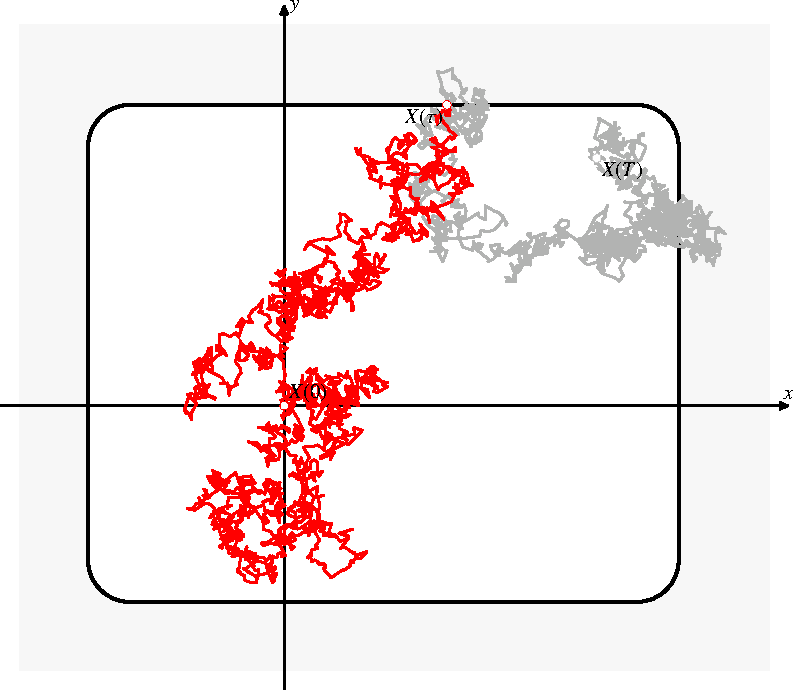
\includegraphics{chapters/images/stochastisch-2.pdf}
\caption{Brownsche Bewegung in zwei Dimension und Definition der
Stopzeit $\tau$, zu der der Pfad $X(t)$ das Gebiet verl"asst.
\label{stochastisch:pfad}}
\end{figure}%
Wie fr"uher betrachten wir wieder einen stochastischen Prozess $X(t)$,
der L"osung einer stochastischen Differentialgleichung
\begin{equation}
\begin{aligned}
dX(t)&=b(t,X)\,dt + B(t,X)\,dW
\\
X(0)&=X_0
\end{aligned}
\label{stochastisch:stopzeitdgl}
\end{equation}
sein soll.

\begin{definition}
Sei $E$ eine beliebige offene oder abgeschlossene nicht leere Teilmenge
von $\mathbb R^n$.
Dann setzen wir
\[
\tau = \inf\{t\ge 0\;|\;X(t)\in E\},
\]
$\tau$ ist also die fr"uheste Zeit, zu der der Weg $X(t)$ die Menge $E$
erreicht.
\end{definition}

Die charakteristische Funktion
\[
\chi_{[0,\tau]}(t)=\begin{cases}
1\qquad\qquad&t\le \tau\\
0            &t>\tau
\end{cases}
\]
ist nat"urlich auch ein stochastischer Prozess, und damit auch 
$\chi_{[0,\tau]}G$.
Damit gelten die Regeln f"ur das It\^o-Integral aus
Satz~\ref{satz:ito-integral} auch f"ur diesen Prozess, jetzt allerdings
als Integrale mit oberer Grenze $\tau$ statt $T$.

\begin{hilfssatz}
Seien $G$ und $H$ auf $[0,T]$ quadratintegrierbare stochastische Prozesse
und $a,b\in\mathbb R$
\begin{compactenum}
\item
Das It\^o-Integral ist linear:
\begin{align*}
\int_0^\tau aG+bH\,dW
&=
\int_0^T a\chi_{[0,\tau]} G + b \chi_{[0,\tau]} H\,dW
=
a\int_0^T \chi_{[0,\tau]} G\,dW + b \int_0^T\chi_{[0,\tau]} H\,dW
\\
&=
a\int_0^\tau G\,dW + b \int_0^\tau H\,dW
\end{align*}
\item Der Erwartungswert des It\^o-Integrals ist
\[
E\biggl(\int_0^\tau G\,dW\biggr)
=
E\biggl(\int_0^T \chi_{[0,\tau]}G\,dW\biggr)
=
0.
\]
\item Die Varianz des It\^o-Integrals ist
\[
E\biggl(\biggl(\int_0^\tau G\,dW\biggr)^2\biggr)
=
E\biggl(\biggl(\int_0^T \chi_{[0,\tau]}G\,dW\biggr)^2\biggr)
=
E\biggl(\int_0^T\chi_{[0,\tau]}G^2\,dt\biggr)
=
E\biggl(\int_0^\tau G^2\,dt\biggr).
\]
\end{compactenum}
\end{hilfssatz}

Die It\^o-sche Kettenregel funktioniert auch f"ur $\tau$ als obere
Grenze f"ur die stochastischen Integrale.
Wenn also $X$ als stochastischer Prozess eine L"osung der stochastischen
Differentialgleichung (\ref{stochastisch:stopzeitdgl}) ist, dann gilt
nach der der It\^o-schen Kettenregel
\[
du(X,t)
=
\frac{\partial u}{\partial t}\,dt
+
\sum_{i=1}^n\frac{\partial u}{\partial x_i}\,dX_i
+
\frac12\sum_{i,j=1}^n\frac{\partial^2 u}{\partial x_i\partial x_j}
\sum_{k=1}^n b_{ik}b_{jk}\,dt.
\]
In integrierter Form bedeutet dies
\[
u(X(t),t)-u(X(0),0)
=
\int_0^t
\frac{\partial u}{\partial t}
+
\frac12\sum_{k=1}^nb_{ik}b_{jk}
\sum_{i,j=1}^n \frac{\partial^2u}{\partial x_i\,\partial x_j} \,ds
+
\int_0^t \operatorname{grad} u\cdot B\,dW.
\]
Und nat"urlich gelten diese Formeln auch dann, wenn man $t$ durch $\tau$
ersetzt.

Im Folgenden interessiert uns nur der Fall $b=0$, $b_{ik}=\delta_{ik}$
und Funktionen $u$, die nicht von der Zeit abh"angen.
Dann vereinfacht sich die Formel zu
\begin{equation}
u(X(t))-u(X(0))
=
\int_0^t \frac12\sum_{i=1}^n\frac{\partial^2 u}{\partial x_i^2}\,ds
=
\int_0^t \frac12\Delta u\,ds
\label{stochastisch:laplaceinkrement}
\end{equation}
Ausserdem ist in diesem Fall $X$ nichts anderes als eine Brownsche Bewegung,
$X=W$.

\subsection{Brownsche Bewegung und der Laplace-Operator}
Wir wenden die Formel (\ref{stochastisch:laplaceinkrement}) jetzt in
zwei Beispielen an.

\subsubsection{Zeit bis zum Verlassen eines Gebietes}
F"ur das erste Beispiel sei $U$ ein beschr"anktes Gebiet in
$\mathbb R^n$, und $u$ eine L"osung der partiellen Differentialgleichung
\begin{equation}
\begin{aligned}
-\frac12\Delta u&=1&\qquad&\text{in $U$}\\
               u&=0&      &\text{auf $\partial U$}
\end{aligned}
\label{stochastisch:hittingtime}
\end{equation}
Wir m"ochten die L"osung $u$ dazu verwenden, die Zeit $\tau_x$ zu berechnen,
zu der eine im Punkt $x\in U$ beginnende Brownsche Bewegung zum ersten
Mal das Gebiet $U$ verl"asst.
Die Formel (\ref{stochastische:laplaceinkrement}) liefert
\[
u(X(\tau_x))-u(X(0)) = \int_0^{\tau_x} \frac12\Delta u\,ds
\]
Da $u$ eine L"osung von (\ref{stochastisch:hittingtime}) ist, ist der 
Integrand auf der rechten Seite gleich $-1$:
\[
u(X(\tau_x))-u(X(0)) = -\int_0^{\tau_x} \,ds
\]
Da der Prozess $X$ zur Zeit $\tau_x$ den Rand des Gebietes "uberquert,
ist wegen der Randbedingung $u(X(\tau_x))=0$. 
Zusammen erhalten wir
\[
-u(X(0)) = -\tau_x.
\]
Nun interessiert uns aber nicht der Wert der Zufallsvariablen, sondern
nur deren Erwartungswert:
\[
E(\tau_x)=E(u(X(0)))=u(x).
\]
Die L"osung $u$ der Differentialgleichung (\ref{stochastisch:hittingtime})
gibt die erwartete Zeit an, bis eine bei $x$ beginnende Brownsche Bewegung 
das Gebiet $U$ verlassen hat.

\subsubsection{Charakterisierung von harmonischen Funktionen}
Sei wieder $U$ ein beschr"anktes Gebiet mit glattem Rand und
$g$ eine stetige Funktion auf $\partial U$.
Ausserdem sei $u$ eine harmonische Funktion in $U$ mit den Randwerten $g$, 
also eine L"osung der partiellen Differentialgleichung
\begin{equation}
\begin{aligned}
\Delta u&=0&\qquad&\text{in $U$}\\
       u&=g&      &\text{auf $\partial U$}
\end{aligned}
\label{stochastisch:harmonisch}
\end{equation}
Wir wollen (\ref{stochastisch:laplaceinkrement}) verwenden, die Funktion
$u$ zu charakterisieren.
Dazu sei wieder $\tau_x$ die Zeit, zu der eine im Punkt $x\in U$ beginnende
Brownsche Bewegung das Gebiet $U$ verl"asst.
Aus (\ref{stochastisch:laplaceinkrement}) folgt:
\[
u(X(\tau_x))-u(X(0))
=
\int_0^{\tau_x} \frac12\underbrace{\Delta u}_{\textstyle=0}\,ds=0.
\]
Zur Zeit $\tau_x$ ist $X(\tau_x)$ ein Randpunkt des Gebiets, der mit
der Randbedingung bestimmt werden kann, es folgt:
\[
u(X(0)) = g(X(\tau_x)).
\]
Wieder interessiert uns der einzelne Wert nicht, sondern der Erwartungswert:
\[
u(x)=E(g(X(\tau_x))).
\]
Den Wert im Punkt $x$ einer harmonischen Funktion mit Randwerten $g$
kann man wie folgt finden: man l"asst eine Brownsche Bewegung von $x$ 
aus laufen, bis sie den Rand "uberquert, und nimmt den Mittelwert
der derart erreichten Randwerte.

Aus dieser Charakterisierung der harmonischen Funktionen kann man
auch deren Mittelwerteigenschaft ableiten. 
Da die Brownsche Bewegung isotrop ist, muss sich im Zentrum
eines kugelf"ormigen Gebietes immer der gleiche Wert f"ur $u$
ergeben, selbst wenn man eine beliebige Drehung auf die Randwerte 
anwendet.
Also muss der Wert von $u(x)$ der Mittelwert der Werte
auf einer Kugel um den Punkt $x$ sein.

%
% kalman.tex -- Anwendung stochastischer DGL auf Kalman Filter
%
\section{Kalman-Filter\label{section:kalman}}
\rhead{Kalman-Filter}
Der klassische diskrete Kalmanfilter l"ost das Filterproblem f"ur ein
diskretes, lineares dynamisches System.
Das System wird mit Hilfe einer linearen Differenzengleichung beschrieben,
in der ein diskreter stochastische Prozess sowohl bei der Systementwicklung
wie auch beim Messen Einfluss nimmt.
Der Filter soll aus den Messungen den Systemzustand rekonstruieren, soweit
dies von den stochastischen Komponenten nicht verunm"oglicht wird.
Der Kalman-Filer l"ost auf optimale Weise: jede andere L"osung hat
eine gr"ossere Fehlervarianz.
Eine detaillierte Darstellung des Filterproblems wird gegeben im
Skript \cite{skript:wrstat}, die dort verwendete Notation wird auch
im Abschnitt~\ref{skript:diskreter-kalman-filter} verwendet.

Es liegt nahe, nach einer entsprechenden L"osung f"ur kontinuierliche
Systeme zu fragen.
Zwar ist es in sehr vielen F"allen in der Praxis m"oglich, dank
Diskretisierung mit dem diskreten Kalman-Filter eine gute L"osung
zu finden.
Dies wird verunm"oglicht wenn die Abtastrate zu gross wird, und die
Rechenleistung f"ur den mathematisch relativ aufwendigen
Kalman-Filter nicht zur Verf"ugung steht.

Die Theorie der stochastischen Differentialgleichungen verallgemeinert
stochastische lineare Differenzengleichungen zu stochastischen
Differentialgleichungen, und erm"oglicht so, das Filter-Problem f"ur
ein kontinuierliches System zu formulieren.
Im Folgenden soll gezeigt werden, wie das Filterproblem formuliert
werden muss, und es soll die L"osung des Filterproblems skizziert werden.
Die L"osung ist nicht vollst"andig, sie wird in einigen F"allen nur durch
Analogie dargestellt, f"ur die Details wird auf die weiterf"uhrende
Literatur verwiesen.
Eine gute Einf"uhrung in das Filterproblem ist das Buch \cite{skript:filter}
von Fridstedt, Jain und Krylow.
Eine detaillierte Untersuchung findet man in Kapitel~6 des Klassikers
\cite{skript:oksendal} von \O{}ksendal.

%
% Beschreibung des diskreten Kalman-Filters zum späteren Vergleich
% des stetigen Problems
%
\subsection{Der diskrete Kalman-Filter\label{skript:diskreter-kalman-filter}}
\index{diskretes Filterproblem}
Das klassische diskrete Filterproblem beschreibt ein System mit Hilfe
eines $n$-dimensionalen Vektors $x_k$ zu diskreten Zeitpunkten, spezifiziert
durch den Index $k$.
Die zeitliche Entwicklung wird durch ein Matrix $\varphi_k$
gem"ass
\begin{equation}
x_{k+1} = \varphi_k x_k + u_k
\label{stochastisch:diskrete-entwicklungs-gleichung}
\end{equation}
beschreiben, jedoch nur bis auf einen normalverteilten Fehler $u_k$.
Gemessen wird aber nicht $x_k$, sondern nur ein Teil oder eine
Linearkombination $H_kx_k$ der Komponenten von $x_k$, und auch wieder
nur mit einem unvermeidbaren normalverteilten Fehler $w_k$:
\[
z_k=H_kx_k + w_k.
\]
Die Aufgabe des Filterproblems besteht darin, die Werte $x_k$ mit m"oglichst
kleinem Fehler zu sch"atzen.
Die gesch"atzten Werte werden mit $\hat x_k$ bezeichnet.

Die L"osung besteht jeweils aus zwei Schritten. 
Zun"achst wird $\varphi_k$ dazu verwendet, eine Sch"atzung $\hat x_{k+1|k}$
des Systemszustand f"ur die Zeit $k+1$ nur auf Grund der zur Zeit
$k$ zur Verf"ugung stehenden Informationen zu bestimmen.
Die Matrix $\varphi_k$ liefert diese Information mittels
\[
\hat x_{k+1|k} = \varphi_k \hat x_k.
\]
Im zweiten Schritt verwendet man die Messung, um den Fehler zu korrigieren.
Dazu wird zun"achst berechnet, was gemessen werden m"usste, wenn
$\hat x_{k+1|k}$ bereits die richtige L"osung w"are.
Die Abweichung der vorhergesagten Messung $H_{k+1}\hat x_{k+1|k}$
von der tats"achlichen Messung $z_{k+1}$ ist
$z_{k+1}-H_{k+1}\hat x_{k+1|k}$r, daraus wird die Korrektur mit Hilfe
der Gain-Matrix $K_{k+1}$ nach
\index{Gain-Matrix}%
\[
\hat x_{k+1}
=
x_{k+1|k} + K_{k+1}(z_{k+1} - H_{k+1} \hat x_{k+1|k})
=
(I-K_{k+1}H_{k+1}) \varphi_{k}\hat x_k + K_{k+1}z_{k+1}
\]
berechnet.
Der Fehler der Sch"atzung $\hat x_{k+1}$ kann mit Hilfe der
Fehler-Kovarianzmatrizen $Q_k=E(u_ku^t_k)$ der Systemfehler $u_k$
\index{Fehler-Kovarianz}
und $R_k=E(w_kw_k^t)$ der Messfehler $w_k$ bestimmt werden.
Die Fehlerkovarianz ist
\begin{align*}
P_{k+1|k}
&=
\varphi_k P_k \varphi_k^t + Q_k
&
&\text{Fehler der Vorhersage}
\\
P_{k+1}
&=
(I-K_{k+1}H_{k+1})P_{k+1|k}(I-K_{k+1}H_{k+1})^t + K_{k+1}R_{k+1}K_{k+1}^t
&
&\text{Fehler nach Korrektur}
\end{align*}
Die optimale L"osung wird f"ur die {\em Kalman-Matrix}
\index{Kalman-Matrix}
\[
K_{k+1}
=
P_{k+1|k}H_{k+1}^t(H_{k+1}P_{k+1|k}H_{k+1}^t + R_{k+1})^{-1}
\]
als Gain-Matrix gefunden, und der Sch"atzfehler ist
\[
P_{k+1}=(I-K_{k+1}H_{k+1})(\varphi_{k}P_k\varphi_k^t+Q_k).
\]

Die L"osung des Filterpoblem in dieser Form ist nicht direkt f"ur ein
kontinuierliches System verallgemeinerungsf"ahig, denn Vorhersage und 
Korrektur erfolgen in dieser zeitlichen Reihenfolge.
Bei einem kontinuierlichen System ist dies nicht m"oglich.
Stattdessen muss Korrektur und Messung sozusagen gleichzeitig erfolgen,
und wir m"ussen erst noch ein mathematische Formulierung daf"ur finden.

%
% Formulierung des stetigen Filterproblems, insbesondere die Formulierung
% als stochastisches Differentialgleichugnssystems, aber auch das Problem
% der bedingten Erwartung.
%
\subsection{Das kontinuierliche Filterproblem}
Wir suchen jetzt eine kontinuierliche Entsprechung f"ur die diskrete
Entwicklungsgleichung~\eqref{stochastisch:diskrete-entwicklungs-gleichung}.
Gesucht ist der zeitabhn"agige $n$-dimensional Systemzustand $X(t)$. 
Die Entwicklung des Systems wird durch eine lineare Differentialgleichung
\[
\frac{dX(t)}{dt}
=
F(t) X(t)
\]
mit einer zeitabh"angigen $n\times n$-Matrix $F(t)$ beschrieben.
Die Entwicklung wird nun aber nicht exakt eingehalten, den Fehler
modellieren wir mit Hilfe eines Wiener-Prozesses.
Dazu m"ussen wir die Differentialgleichung jedoch wieder in Inkrementform
schreiben:
\begin{equation}
dX(t) = F(t) X(t)\,dt + C(t)\, dU(t),
\label{stochastisch:kontinuierliche-zeitentwicklung}
\end{equation}
worin $U(t)$ ein $n$-dimensionaler Wiener-Prozess ist und $C(t)$
eine $n\times n$-Matrix.

Nun ist aber nicht $X(t)$ bekannt, sondern nur eine $m$-dimensionale
Messung $Z(t)$, die jedoch auch nicht exakt ist.
Die Messung h"angt linear vom Systemzustand ab, es gibt also eine
$m\times n$-Matrix $G(t)$ mit 
\[
Z(t) = G(t) X(t).
\]
Der Matrix $G(t)$ entspricht im diskreten Filterproblem die Matrix $H_k$.

Wir m"ussen jetzt aber noch den Messfehler modellieren.
Dieser sollte im Wesentlichen ein Wiener-Prozess sein, wir k"onnen daher
den Messprozess durch die stochastische Differentialgleichung
\begin{equation}
dZ(t)
= 
G(t)X(t) \,dt +  D(t)\,dV(t)
\label{stochastisch:kontinuierlicher-messprozess}
\end{equation}
beschreiben,
worin $V(t)$ ein $m$-dimensionaler Wiener-Prozess ist und $D(t)$ 
eine $m\times m$-Matrix.

Den Prozess $X(t)$ k"onnen wir grunds"atzlich nicht kennen, sondern
nur eine Sch"atzung $\hat X(t)$ davon.
Die Filter-Aufgabe besteht also darin, einen Prozess $\hat X(t)$ zu
finden mit den folgenden Eigenschaften:
\begin{enumerate}
\item
Die Sch"atzung $\hat X(t)$ ist im Mittel richtig:
$E(\hat X(t)) = E(X(t))$.
\item
$\hat X(t)$ h"angt nur von Messungen $Z(s)$ f"ur $s\le t$ ab.
\item
Unter allen Sch"atzprozessen $Y(t)$ mit den Eigenschaften 1 und 2 ist
$\hat X(t)$ derjenige, f"ur den der quadratische Fehler 
$E((Y(t)-\hat X(t))^2)$  minimal wird.
\end{enumerate}
Im Folgenden soll versucht werden, eine L"osung des Filterproblems zu
finden.

%
% Lösung des Filterproblems nach Kalman-Bucy, insbesondere die Entwicklung
% des Fehlers (Riccati-Differentialgleichung)
%
\subsection{L"osung des Filterproblems\label{stochastisch:loesung-filterproblem}}
In diesem Abschnitt beschreiben wir die L"osung des Filterproblems
f"ur den eindimensionalen Fall ($n=m=1$).

Ohne die Information aus dem Messprozess $Z(t)$ steht f"ur die 
Sch"atzung nur noch die
Entwicklungsgleichung~\eqref{stochastisch:kontinuierliche-zeitentwicklung}
zur Verf"ugung.
Ausserdem ist der Systemfehler unbekannt, so dass nur noch die gew"ohnliche
lineare Differentialgleichung
\begin{equation}
d\hat X(t) = F(t)\hat X(t)\,dt
\label{stochastisch:homogene-entwicklung}
\end{equation}
bleibt.

Die Gleichung~\eqref{stochastisch:homogene-entwicklung} muss erweitert
werden um einen Term, der die Abweichung der Messung misst.
Ohne die Messfehler m"usste
\[
dZ(t) = G(t)\hat X(t)\,dt
\]
sein.
Als Basis f"ur die Korrektur muss die Differenz zur tats"achlichen
Messung verwendet werden, also
\begin{equation}
dN(t)
=
dZ(t) - G(t)\hat X(t)\,dt
=
G(t)(X(t)-\hat X(t))\,dt + D(t)\,dV(t)
.
\label{stochastisch:innovations-prozess}
\end{equation}
Die Korrektur muss linear von \eqref{stochastisch:innovations-prozess}
abh"angen, die stochastische Differentialgleichung f"ur $\hat X(t)$
hat daher die Form
\begin{align*}
d\hat X(t)
&=
F(t)\hat X(t)\,dt + K(t)\,dN(t),
\\
&=
F(t)\hat X(t)\,dt
+
K(t)\,dZ(t) - K(t)G(t)\hat X(t)\,dt
\\
&=
(F(t)-K(t)G(t))\hat X(t)\,dt
+
K(t)\,dZ(t)
\end{align*}
mit einer noch zu bestimmenden Funktionen $K(t)$.
$N(t)$ heisst der Innovations-Prozess.
Die Funktion $K(t)$ muss so bestimmt werden, dass die Bedingungen
1--3 an den Sch"atzprozess erf"ullt sind.

Der Sch"atzfehler zur Zeit $t$ ist der Erwartungswert
\[
S(t) = E((X(t)-\hat X(T))^2).
\]
Man kann zeigen, dass $S(t)$ die gew"ohnliche Differentialgleichung
\begin{equation}
\frac{dS}{dt}
=
2F(t)S(t) - \frac{G(t)^2}{D(t)^2}S(t)^2 +C(t)^2
\label{stochastisch:ricatti}
\end{equation}
erf"ullt.
\eqref{stochastisch:ricatti} ist eine Riccati-Differentialgleichung.
Mit $S(t)$ kann das Filterproblem gel"ost werden, es gilt
\begin{equation}
d\hat X(t)
=
\biggl(F(t)-\frac{G(t)^2S(t)}{D(t)^2}\biggr)\hat X(t)\,dt 
+
\frac{G(t)S(t)}{D(t)^2}\,dZ(t).
\end{equation}











